
\documentclass{article} % For LaTeX2e
\PassOptionsToPackage{table}{xcolor}
\usepackage{iclr2027_conference,times}

% Optional math commands from https://github.com/goodfeli/dlbook_notation.
%%%%% NEW MATH DEFINITIONS %%%%%

\usepackage{amsmath,amsfonts,bm}

% Mark sections of captions for referring to divisions of figures
\newcommand{\figleft}{{\em (Left)}}
\newcommand{\figcenter}{{\em (Center)}}
\newcommand{\figright}{{\em (Right)}}
\newcommand{\figtop}{{\em (Top)}}
\newcommand{\figbottom}{{\em (Bottom)}}
\newcommand{\captiona}{{\em (a)}}
\newcommand{\captionb}{{\em (b)}}
\newcommand{\captionc}{{\em (c)}}
\newcommand{\captiond}{{\em (d)}}

% Highlight a newly defined term
\newcommand{\newterm}[1]{{\bf #1}}


% Figure reference, lower-case.
\def\figref#1{figure~\ref{#1}}
% Figure reference, capital. For start of sentence
\def\Figref#1{Figure~\ref{#1}}
\def\twofigref#1#2{figures \ref{#1} and \ref{#2}}
\def\quadfigref#1#2#3#4{figures \ref{#1}, \ref{#2}, \ref{#3} and \ref{#4}}
% Section reference, lower-case.
\def\secref#1{section~\ref{#1}}
% Section reference, capital.
\def\Secref#1{Section~\ref{#1}}
% Reference to two sections.
\def\twosecrefs#1#2{sections \ref{#1} and \ref{#2}}
% Reference to three sections.
\def\secrefs#1#2#3{sections \ref{#1}, \ref{#2} and \ref{#3}}
% Reference to an equation, lower-case.
\def\eqref#1{equation~\ref{#1}}
% Reference to an equation, upper case
\def\Eqref#1{Equation~\ref{#1}}
% A raw reference to an equation---avoid using if possible
\def\plaineqref#1{\ref{#1}}
% Reference to a chapter, lower-case.
\def\chapref#1{chapter~\ref{#1}}
% Reference to an equation, upper case.
\def\Chapref#1{Chapter~\ref{#1}}
% Reference to a range of chapters
\def\rangechapref#1#2{chapters\ref{#1}--\ref{#2}}
% Reference to an algorithm, lower-case.
\def\algref#1{algorithm~\ref{#1}}
% Reference to an algorithm, upper case.
\def\Algref#1{Algorithm~\ref{#1}}
\def\twoalgref#1#2{algorithms \ref{#1} and \ref{#2}}
\def\Twoalgref#1#2{Algorithms \ref{#1} and \ref{#2}}
% Reference to a part, lower case
\def\partref#1{part~\ref{#1}}
% Reference to a part, upper case
\def\Partref#1{Part~\ref{#1}}
\def\twopartref#1#2{parts \ref{#1} and \ref{#2}}

\def\ceil#1{\lceil #1 \rceil}
\def\floor#1{\lfloor #1 \rfloor}
\def\1{\bm{1}}
\newcommand{\train}{\mathcal{D}}
\newcommand{\valid}{\mathcal{D_{\mathrm{valid}}}}
\newcommand{\test}{\mathcal{D_{\mathrm{test}}}}

\def\eps{{\epsilon}}


% Random variables
\def\reta{{\textnormal{$\eta$}}}
\def\ra{{\textnormal{a}}}
\def\rb{{\textnormal{b}}}
\def\rc{{\textnormal{c}}}
\def\rd{{\textnormal{d}}}
\def\re{{\textnormal{e}}}
\def\rf{{\textnormal{f}}}
\def\rg{{\textnormal{g}}}
\def\rh{{\textnormal{h}}}
\def\ri{{\textnormal{i}}}
\def\rj{{\textnormal{j}}}
\def\rk{{\textnormal{k}}}
\def\rl{{\textnormal{l}}}
% rm is already a command, just don't name any random variables m
\def\rn{{\textnormal{n}}}
\def\ro{{\textnormal{o}}}
\def\rp{{\textnormal{p}}}
\def\rq{{\textnormal{q}}}
\def\rr{{\textnormal{r}}}
\def\rs{{\textnormal{s}}}
\def\rt{{\textnormal{t}}}
\def\ru{{\textnormal{u}}}
\def\rv{{\textnormal{v}}}
\def\rw{{\textnormal{w}}}
\def\rx{{\textnormal{x}}}
\def\ry{{\textnormal{y}}}
\def\rz{{\textnormal{z}}}

% Random vectors
\def\rvepsilon{{\mathbf{\epsilon}}}
\def\rvtheta{{\mathbf{\theta}}}
\def\rva{{\mathbf{a}}}
\def\rvb{{\mathbf{b}}}
\def\rvc{{\mathbf{c}}}
\def\rvd{{\mathbf{d}}}
\def\rve{{\mathbf{e}}}
\def\rvf{{\mathbf{f}}}
\def\rvg{{\mathbf{g}}}
\def\rvh{{\mathbf{h}}}
\def\rvu{{\mathbf{i}}}
\def\rvj{{\mathbf{j}}}
\def\rvk{{\mathbf{k}}}
\def\rvl{{\mathbf{l}}}
\def\rvm{{\mathbf{m}}}
\def\rvn{{\mathbf{n}}}
\def\rvo{{\mathbf{o}}}
\def\rvp{{\mathbf{p}}}
\def\rvq{{\mathbf{q}}}
\def\rvr{{\mathbf{r}}}
\def\rvs{{\mathbf{s}}}
\def\rvt{{\mathbf{t}}}
\def\rvu{{\mathbf{u}}}
\def\rvv{{\mathbf{v}}}
\def\rvw{{\mathbf{w}}}
\def\rvx{{\mathbf{x}}}
\def\rvy{{\mathbf{y}}}
\def\rvz{{\mathbf{z}}}

% Elements of random vectors
\def\erva{{\textnormal{a}}}
\def\ervb{{\textnormal{b}}}
\def\ervc{{\textnormal{c}}}
\def\ervd{{\textnormal{d}}}
\def\erve{{\textnormal{e}}}
\def\ervf{{\textnormal{f}}}
\def\ervg{{\textnormal{g}}}
\def\ervh{{\textnormal{h}}}
\def\ervi{{\textnormal{i}}}
\def\ervj{{\textnormal{j}}}
\def\ervk{{\textnormal{k}}}
\def\ervl{{\textnormal{l}}}
\def\ervm{{\textnormal{m}}}
\def\ervn{{\textnormal{n}}}
\def\ervo{{\textnormal{o}}}
\def\ervp{{\textnormal{p}}}
\def\ervq{{\textnormal{q}}}
\def\ervr{{\textnormal{r}}}
\def\ervs{{\textnormal{s}}}
\def\ervt{{\textnormal{t}}}
\def\ervu{{\textnormal{u}}}
\def\ervv{{\textnormal{v}}}
\def\ervw{{\textnormal{w}}}
\def\ervx{{\textnormal{x}}}
\def\ervy{{\textnormal{y}}}
\def\ervz{{\textnormal{z}}}

% Random matrices
\def\rmA{{\mathbf{A}}}
\def\rmB{{\mathbf{B}}}
\def\rmC{{\mathbf{C}}}
\def\rmD{{\mathbf{D}}}
\def\rmE{{\mathbf{E}}}
\def\rmF{{\mathbf{F}}}
\def\rmG{{\mathbf{G}}}
\def\rmH{{\mathbf{H}}}
\def\rmI{{\mathbf{I}}}
\def\rmJ{{\mathbf{J}}}
\def\rmK{{\mathbf{K}}}
\def\rmL{{\mathbf{L}}}
\def\rmM{{\mathbf{M}}}
\def\rmN{{\mathbf{N}}}
\def\rmO{{\mathbf{O}}}
\def\rmP{{\mathbf{P}}}
\def\rmQ{{\mathbf{Q}}}
\def\rmR{{\mathbf{R}}}
\def\rmS{{\mathbf{S}}}
\def\rmT{{\mathbf{T}}}
\def\rmU{{\mathbf{U}}}
\def\rmV{{\mathbf{V}}}
\def\rmW{{\mathbf{W}}}
\def\rmX{{\mathbf{X}}}
\def\rmY{{\mathbf{Y}}}
\def\rmZ{{\mathbf{Z}}}

% Elements of random matrices
\def\ermA{{\textnormal{A}}}
\def\ermB{{\textnormal{B}}}
\def\ermC{{\textnormal{C}}}
\def\ermD{{\textnormal{D}}}
\def\ermE{{\textnormal{E}}}
\def\ermF{{\textnormal{F}}}
\def\ermG{{\textnormal{G}}}
\def\ermH{{\textnormal{H}}}
\def\ermI{{\textnormal{I}}}
\def\ermJ{{\textnormal{J}}}
\def\ermK{{\textnormal{K}}}
\def\ermL{{\textnormal{L}}}
\def\ermM{{\textnormal{M}}}
\def\ermN{{\textnormal{N}}}
\def\ermO{{\textnormal{O}}}
\def\ermP{{\textnormal{P}}}
\def\ermQ{{\textnormal{Q}}}
\def\ermR{{\textnormal{R}}}
\def\ermS{{\textnormal{S}}}
\def\ermT{{\textnormal{T}}}
\def\ermU{{\textnormal{U}}}
\def\ermV{{\textnormal{V}}}
\def\ermW{{\textnormal{W}}}
\def\ermX{{\textnormal{X}}}
\def\ermY{{\textnormal{Y}}}
\def\ermZ{{\textnormal{Z}}}

% Vectors
\def\vzero{{\bm{0}}}
\def\vone{{\bm{1}}}
\def\vmu{{\bm{\mu}}}
\def\vtheta{{\bm{\theta}}}
\def\va{{\bm{a}}}
\def\vb{{\bm{b}}}
\def\vc{{\bm{c}}}
\def\vd{{\bm{d}}}
\def\ve{{\bm{e}}}
\def\vf{{\bm{f}}}
\def\vg{{\bm{g}}}
\def\vh{{\bm{h}}}
\def\vi{{\bm{i}}}
\def\vj{{\bm{j}}}
\def\vk{{\bm{k}}}
\def\vl{{\bm{l}}}
\def\vm{{\bm{m}}}
\def\vn{{\bm{n}}}
\def\vo{{\bm{o}}}
\def\vp{{\bm{p}}}
\def\vq{{\bm{q}}}
\def\vr{{\bm{r}}}
\def\vs{{\bm{s}}}
\def\vt{{\bm{t}}}
\def\vu{{\bm{u}}}
\def\vv{{\bm{v}}}
\def\vw{{\bm{w}}}
\def\vx{{\bm{x}}}
\def\vy{{\bm{y}}}
\def\vz{{\bm{z}}}

% Elements of vectors
\def\evalpha{{\alpha}}
\def\evbeta{{\beta}}
\def\evepsilon{{\epsilon}}
\def\evlambda{{\lambda}}
\def\evomega{{\omega}}
\def\evmu{{\mu}}
\def\evpsi{{\psi}}
\def\evsigma{{\sigma}}
\def\evtheta{{\theta}}
\def\eva{{a}}
\def\evb{{b}}
\def\evc{{c}}
\def\evd{{d}}
\def\eve{{e}}
\def\evf{{f}}
\def\evg{{g}}
\def\evh{{h}}
\def\evi{{i}}
\def\evj{{j}}
\def\evk{{k}}
\def\evl{{l}}
\def\evm{{m}}
\def\evn{{n}}
\def\evo{{o}}
\def\evp{{p}}
\def\evq{{q}}
\def\evr{{r}}
\def\evs{{s}}
\def\evt{{t}}
\def\evu{{u}}
\def\evv{{v}}
\def\evw{{w}}
\def\evx{{x}}
\def\evy{{y}}
\def\evz{{z}}

% Matrix
\def\mA{{\bm{A}}}
\def\mB{{\bm{B}}}
\def\mC{{\bm{C}}}
\def\mD{{\bm{D}}}
\def\mE{{\bm{E}}}
\def\mF{{\bm{F}}}
\def\mG{{\bm{G}}}
\def\mH{{\bm{H}}}
\def\mI{{\bm{I}}}
\def\mJ{{\bm{J}}}
\def\mK{{\bm{K}}}
\def\mL{{\bm{L}}}
\def\mM{{\bm{M}}}
\def\mN{{\bm{N}}}
\def\mO{{\bm{O}}}
\def\mP{{\bm{P}}}
\def\mQ{{\bm{Q}}}
\def\mR{{\bm{R}}}
\def\mS{{\bm{S}}}
\def\mT{{\bm{T}}}
\def\mU{{\bm{U}}}
\def\mV{{\bm{V}}}
\def\mW{{\bm{W}}}
\def\mX{{\bm{X}}}
\def\mY{{\bm{Y}}}
\def\mZ{{\bm{Z}}}
\def\mBeta{{\bm{\beta}}}
\def\mPhi{{\bm{\Phi}}}
\def\mLambda{{\bm{\Lambda}}}
\def\mSigma{{\bm{\Sigma}}}

% Tensor
\DeclareMathAlphabet{\mathsfit}{\encodingdefault}{\sfdefault}{m}{sl}
\SetMathAlphabet{\mathsfit}{bold}{\encodingdefault}{\sfdefault}{bx}{n}
\newcommand{\tens}[1]{\bm{\mathsfit{#1}}}
\def\tA{{\tens{A}}}
\def\tB{{\tens{B}}}
\def\tC{{\tens{C}}}
\def\tD{{\tens{D}}}
\def\tE{{\tens{E}}}
\def\tF{{\tens{F}}}
\def\tG{{\tens{G}}}
\def\tH{{\tens{H}}}
\def\tI{{\tens{I}}}
\def\tJ{{\tens{J}}}
\def\tK{{\tens{K}}}
\def\tL{{\tens{L}}}
\def\tM{{\tens{M}}}
\def\tN{{\tens{N}}}
\def\tO{{\tens{O}}}
\def\tP{{\tens{P}}}
\def\tQ{{\tens{Q}}}
\def\tR{{\tens{R}}}
\def\tS{{\tens{S}}}
\def\tT{{\tens{T}}}
\def\tU{{\tens{U}}}
\def\tV{{\tens{V}}}
\def\tW{{\tens{W}}}
\def\tX{{\tens{X}}}
\def\tY{{\tens{Y}}}
\def\tZ{{\tens{Z}}}


% Graph
\def\gA{{\mathcal{A}}}
\def\gB{{\mathcal{B}}}
\def\gC{{\mathcal{C}}}
\def\gD{{\mathcal{D}}}
\def\gE{{\mathcal{E}}}
\def\gF{{\mathcal{F}}}
\def\gG{{\mathcal{G}}}
\def\gH{{\mathcal{H}}}
\def\gI{{\mathcal{I}}}
\def\gJ{{\mathcal{J}}}
\def\gK{{\mathcal{K}}}
\def\gL{{\mathcal{L}}}
\def\gM{{\mathcal{M}}}
\def\gN{{\mathcal{N}}}
\def\gO{{\mathcal{O}}}
\def\gP{{\mathcal{P}}}
\def\gQ{{\mathcal{Q}}}
\def\gR{{\mathcal{R}}}
\def\gS{{\mathcal{S}}}
\def\gT{{\mathcal{T}}}
\def\gU{{\mathcal{U}}}
\def\gV{{\mathcal{V}}}
\def\gW{{\mathcal{W}}}
\def\gX{{\mathcal{X}}}
\def\gY{{\mathcal{Y}}}
\def\gZ{{\mathcal{Z}}}

% Sets
\def\sA{{\mathbb{A}}}
\def\sB{{\mathbb{B}}}
\def\sC{{\mathbb{C}}}
\def\sD{{\mathbb{D}}}
% Don't use a set called E, because this would be the same as our symbol
% for expectation.
\def\sF{{\mathbb{F}}}
\def\sG{{\mathbb{G}}}
\def\sH{{\mathbb{H}}}
\def\sI{{\mathbb{I}}}
\def\sJ{{\mathbb{J}}}
\def\sK{{\mathbb{K}}}
\def\sL{{\mathbb{L}}}
\def\sM{{\mathbb{M}}}
\def\sN{{\mathbb{N}}}
\def\sO{{\mathbb{O}}}
\def\sP{{\mathbb{P}}}
\def\sQ{{\mathbb{Q}}}
\def\sR{{\mathbb{R}}}
\def\sS{{\mathbb{S}}}
\def\sT{{\mathbb{T}}}
\def\sU{{\mathbb{U}}}
\def\sV{{\mathbb{V}}}
\def\sW{{\mathbb{W}}}
\def\sX{{\mathbb{X}}}
\def\sY{{\mathbb{Y}}}
\def\sZ{{\mathbb{Z}}}

% Entries of a matrix
\def\emLambda{{\Lambda}}
\def\emA{{A}}
\def\emB{{B}}
\def\emC{{C}}
\def\emD{{D}}
\def\emE{{E}}
\def\emF{{F}}
\def\emG{{G}}
\def\emH{{H}}
\def\emI{{I}}
\def\emJ{{J}}
\def\emK{{K}}
\def\emL{{L}}
\def\emM{{M}}
\def\emN{{N}}
\def\emO{{O}}
\def\emP{{P}}
\def\emQ{{Q}}
\def\emR{{R}}
\def\emS{{S}}
\def\emT{{T}}
\def\emU{{U}}
\def\emV{{V}}
\def\emW{{W}}
\def\emX{{X}}
\def\emY{{Y}}
\def\emZ{{Z}}
\def\emSigma{{\Sigma}}

% entries of a tensor
% Same font as tensor, without \bm wrapper
\newcommand{\etens}[1]{\mathsfit{#1}}
\def\etLambda{{\etens{\Lambda}}}
\def\etA{{\etens{A}}}
\def\etB{{\etens{B}}}
\def\etC{{\etens{C}}}
\def\etD{{\etens{D}}}
\def\etE{{\etens{E}}}
\def\etF{{\etens{F}}}
\def\etG{{\etens{G}}}
\def\etH{{\etens{H}}}
\def\etI{{\etens{I}}}
\def\etJ{{\etens{J}}}
\def\etK{{\etens{K}}}
\def\etL{{\etens{L}}}
\def\etM{{\etens{M}}}
\def\etN{{\etens{N}}}
\def\etO{{\etens{O}}}
\def\etP{{\etens{P}}}
\def\etQ{{\etens{Q}}}
\def\etR{{\etens{R}}}
\def\etS{{\etens{S}}}
\def\etT{{\etens{T}}}
\def\etU{{\etens{U}}}
\def\etV{{\etens{V}}}
\def\etW{{\etens{W}}}
\def\etX{{\etens{X}}}
\def\etY{{\etens{Y}}}
\def\etZ{{\etens{Z}}}

% The true underlying data generating distribution
\newcommand{\pdata}{p_{\rm{data}}}
% The empirical distribution defined by the training set
\newcommand{\ptrain}{\hat{p}_{\rm{data}}}
\newcommand{\Ptrain}{\hat{P}_{\rm{data}}}
% The model distribution
\newcommand{\pmodel}{p_{\rm{model}}}
\newcommand{\Pmodel}{P_{\rm{model}}}
\newcommand{\ptildemodel}{\tilde{p}_{\rm{model}}}
% Stochastic autoencoder distributions
\newcommand{\pencode}{p_{\rm{encoder}}}
\newcommand{\pdecode}{p_{\rm{decoder}}}
\newcommand{\precons}{p_{\rm{reconstruct}}}

\newcommand{\laplace}{\mathrm{Laplace}} % Laplace distribution

\newcommand{\E}{\mathbb{E}}
\newcommand{\Ls}{\mathcal{L}}
\newcommand{\R}{\mathbb{R}}
\newcommand{\emp}{\tilde{p}}
\newcommand{\lr}{\alpha}
\newcommand{\reg}{\lambda}
\newcommand{\rect}{\mathrm{rectifier}}
\newcommand{\softmax}{\mathrm{softmax}}
\newcommand{\sigmoid}{\sigma}
\newcommand{\softplus}{\zeta}
\newcommand{\KL}{D_{\mathrm{KL}}}
\newcommand{\Var}{\mathrm{Var}}
\newcommand{\standarderror}{\mathrm{SE}}
\newcommand{\Cov}{\mathrm{Cov}}
% Wolfram Mathworld says $L^2$ is for function spaces and $\ell^2$ is for vectors
% But then they seem to use $L^2$ for vectors throughout the site, and so does
% wikipedia.
\newcommand{\normlzero}{L^0}
\newcommand{\normlone}{L^1}
\newcommand{\normltwo}{L^2}
\newcommand{\normlp}{L^p}
\newcommand{\normmax}{L^\infty}

\newcommand{\parents}{Pa} % See usage in notation.tex. Chosen to match Daphne's book.

\DeclareMathOperator*{\argmax}{arg\,max}
\DeclareMathOperator*{\argmin}{arg\,min}

\DeclareMathOperator{\sign}{sign}
\DeclareMathOperator{\Tr}{Tr}
\let\ab\allowbreak

% Vector macros used in the Method section that math_commands.tex does not define
\providecommand{\vphi}{{\bm{\phi}}}
\providecommand{\vDelta}{{\bm{\Delta}}}

\usepackage{hyperref}
\usepackage{url}
\usepackage{graphicx}
\usepackage{booktabs}
\usepackage{amssymb}
\usepackage{multirow}
\usepackage{float}   % [H] placement for selected appendix examples

\graphicspath{{figures/}}

\title{Sparse Trajectory Tokens for Metric Motion Queries in Multimodal Language Models}

% Authors must not appear in the submitted version. They should be hidden
% as long as the \iclrfinalcopy macro remains commented out below.
% Non-anonymous submissions will be rejected without review.

\author{Anonymous authors \\
Paper under double-blind review
}

% The \author macro works with any number of authors. There are two commands
% used to separate the names and addresses of multiple authors: \And and \AND.
%
% Using \And between authors leaves it to \LaTeX{} to determine where to break
% the lines. Using \AND forces a linebreak at that point. So, if \LaTeX{}
% puts 3 of 4 authors names on the first line, and the last on the second
% line, try using \AND instead of \And before the third author name.

%\iclrfinalcopy % Uncomment for camera-ready version, but NOT for submission.
\begin{document}


\maketitle

\begin{abstract}
Video-language models can recognize motion yet struggle to answer questions about
metric displacement and motion rate when scale and camera motion must be inferred from
images. We study an interface that supplies an MLLM with externally reconstructed
3D object and camera trajectories alongside video. Our representation associates
sparse, part-aware keypoints with metric world-frame tracks, splits tracks at
occlusions and motion events, and encodes adaptively fitted spline samples as
trajectory tokens. A lightweight projector injects these tokens into
Qwen3-VL-8B without modifying its vision encoder. We also construct TrajQA-B
from Stereo4D tracks, with token-side answer checks and controls for text and
option shortcuts. On its 7,500 four-choice numeric
questions, the trajectory model obtains 82.2\% accuracy, versus 48.3\% for a
separately fine-tuned frames-only reference without timestamps or guaranteed query frames. Replacing trajectories with those of another
scene lowers accuracy to 29.6\%; the model's generated metric evidence also
tracks the reference positions and motion quantities. These results show
dependence on supplied trajectories for these QA tasks. Caption and QA training
exclude the evaluation scenes; source-video separation for caption training
has not been audited. The benchmark uses reconstructed rather than independently
measured motion references.
\end{abstract}

\section{Introduction}
\label{sec:intro}

\begin{figure}[t]
\centering
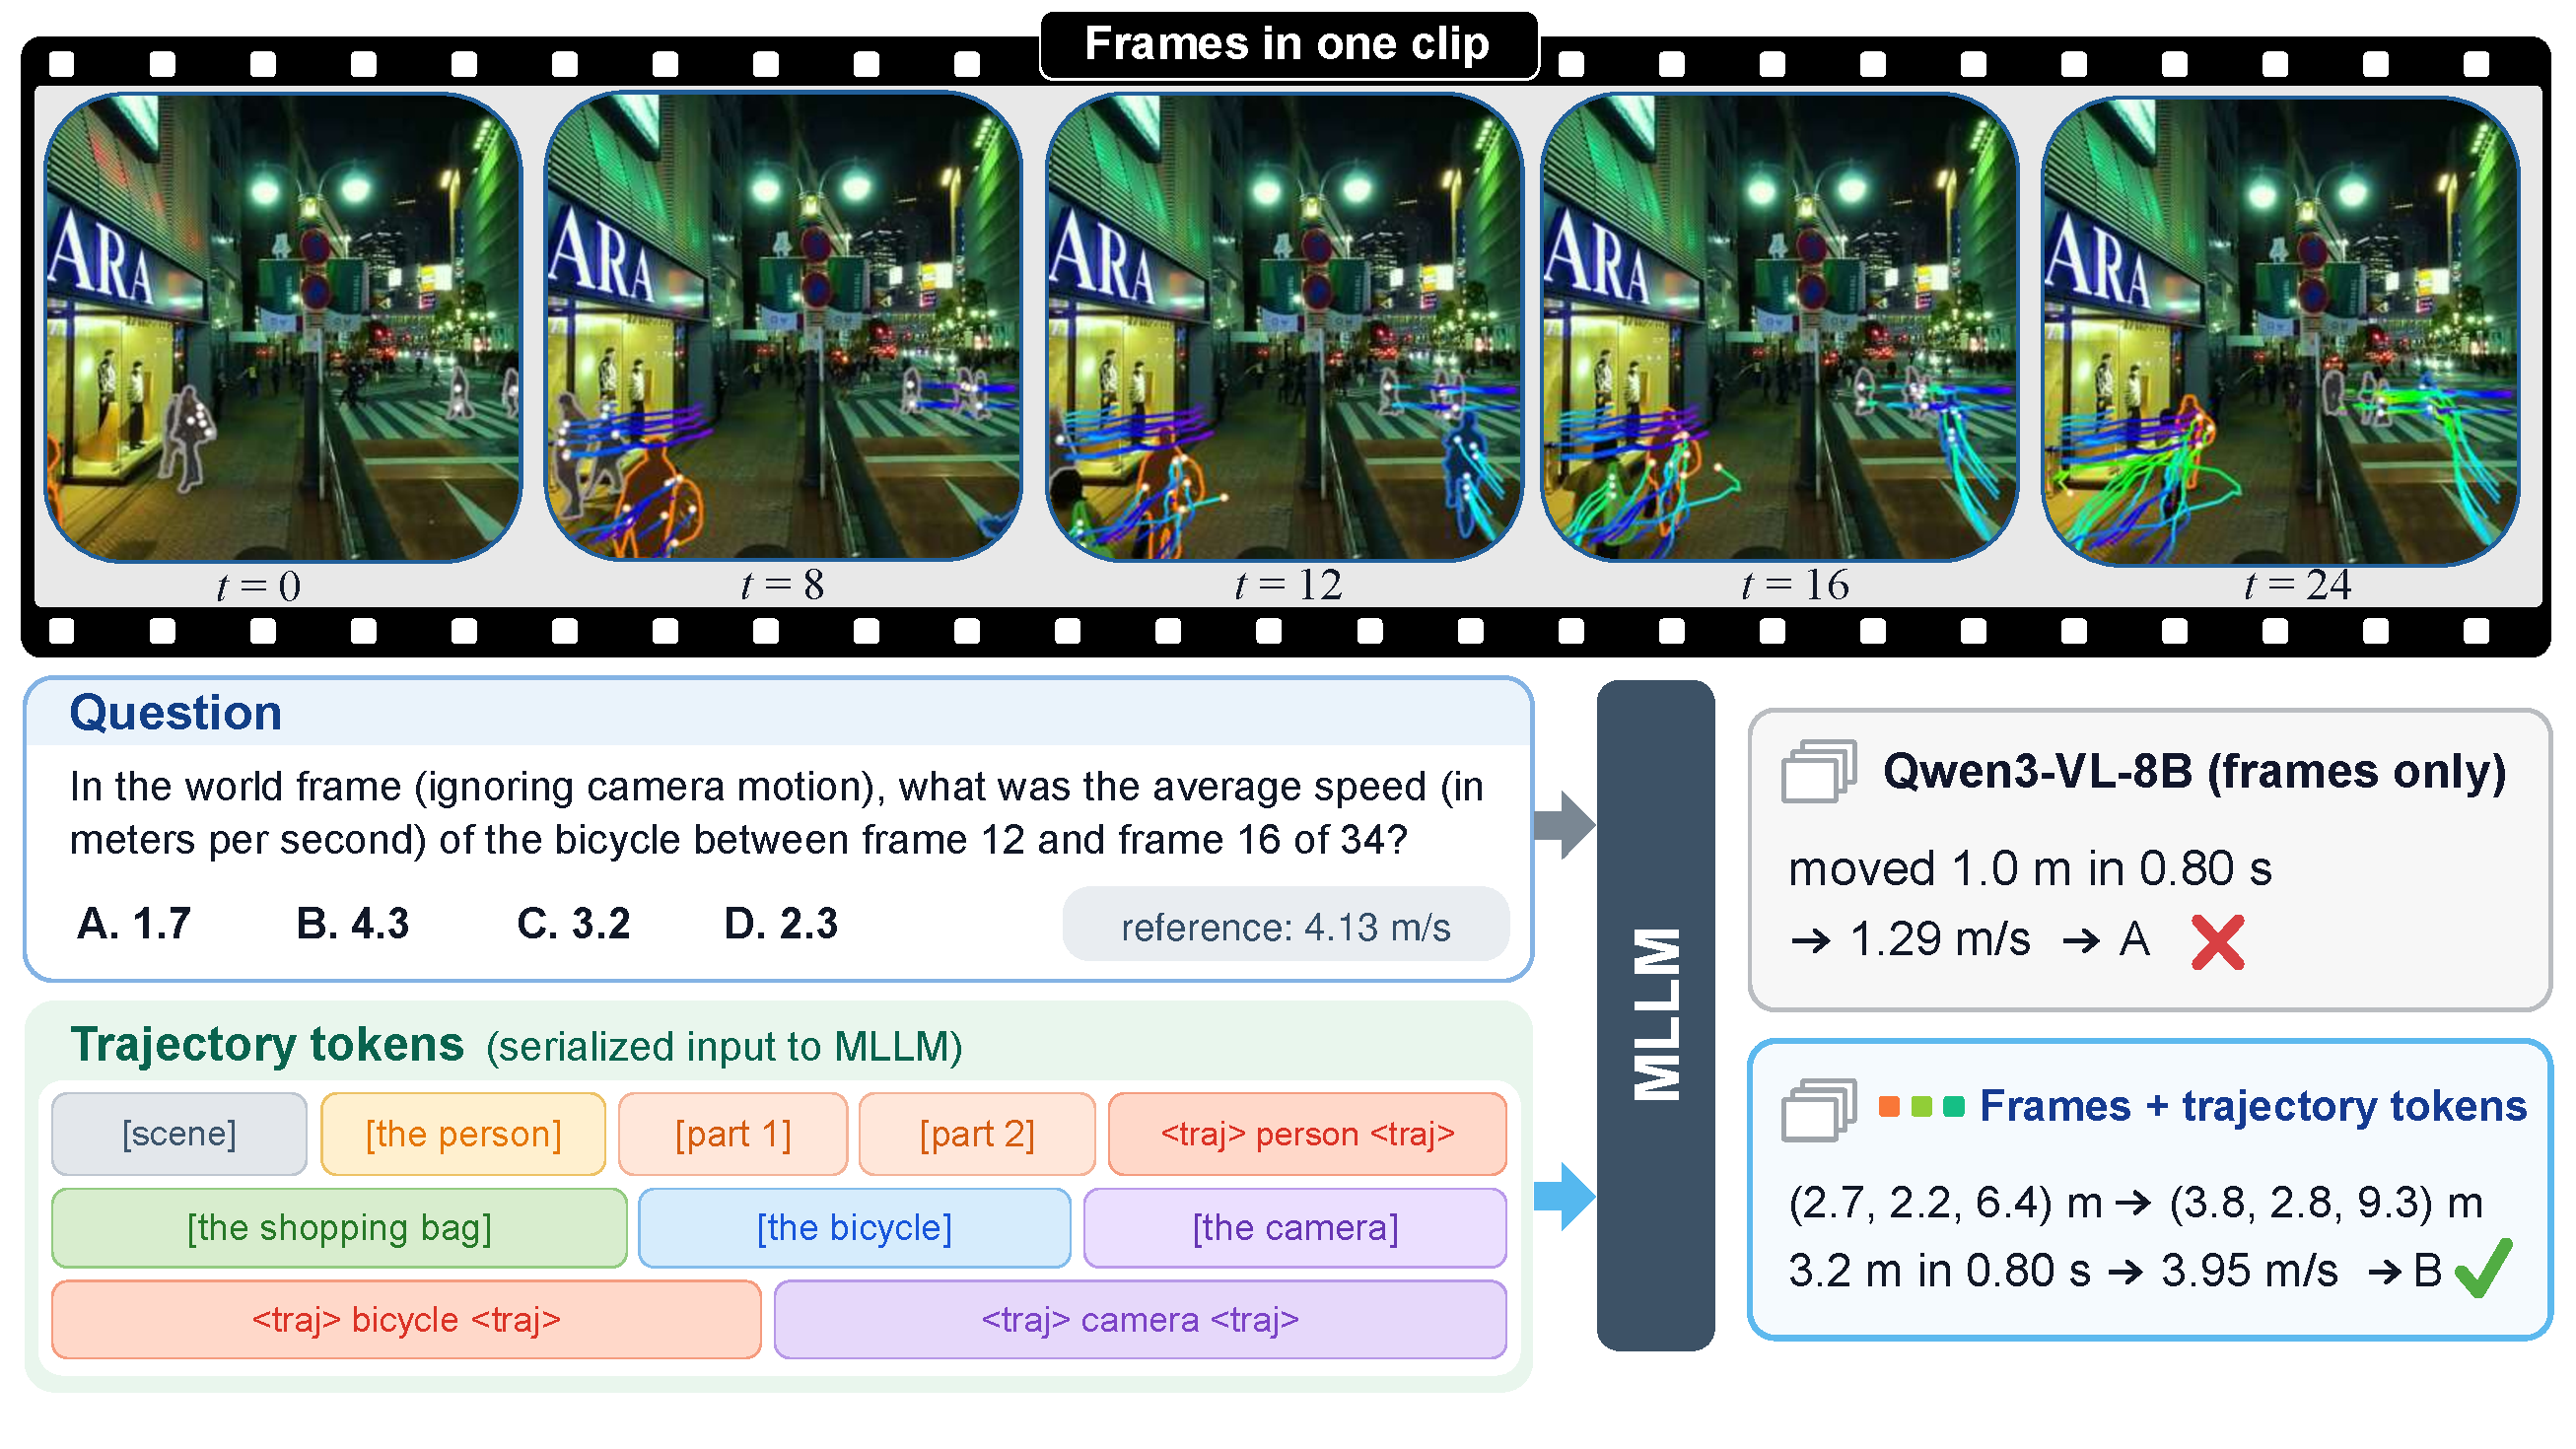
\includegraphics[width=\linewidth]{fig1_teaser_labels.pdf}
\caption{\textbf{Metric motion is hard to read from sampled frames.} Five frames and reconstructed 3D tracks accompany a question whose legacy \emph{average speed} wording is scored as endpoint displacement per elapsed second. Separately fine-tuned Qwen3-VL-8B arms predict 1.29~m/s from frames and 3.95~m/s from frames plus trajectory tokens; the reconstruction-derived reference is 4.13~m/s. The example illustrates the input setting, not an isolated causal effect of any one tokenization component.}
\label{fig:teaser}
\end{figure}

Understanding a dynamic scene requires reasoning about where objects are in three dimensions and how their positions change over physical time. A question such as \emph{How far did the person move between these frames?} needs metric scale, object identity, temporal correspondence, and separation of object motion from camera motion. These quantities matter for embodied agents, video search, and assistive scene understanding, but can be ambiguous in a short, sparsely sampled video. Contemporary multimodal language models (MLLMs) remain weak on spatial and spatiotemporal questions~\citep{yangThinkingSpaceHow2025,jiaOmniSpatialComprehensiveSpatial2026,liViSTRBenchCanMLLMs2026}. Figure~\ref{fig:teaser} shows the particular difficulty of recovering a numerical motion quantity from frames alone.

Most spatial MLLMs acquire geometric knowledge through images, depth, or video instruction tuning~\citep{chenSpatialVLMEndowingVisionLanguage2024,chengSpatialRGPTGroundedSpatial2024,caiSpatialBotPreciseSpatial2025}. Recent dynamic-scene models also incorporate reconstructed features or 4D questions~\citep{fanVLM3RVisionLanguageModels2026,yinMLLM4DVisualbasedSpatialTemporal2026}. Yet the model must still infer and retain the queried world-frame trajectory from a limited visual context. Conversely, 3D reconstruction can supply explicit point tracks, but naively listing hundreds of points across tens of frames overwhelms the language context and obscures which motion belongs to which object. This leaves an interface problem: how can an MLLM read compact, metric, object-grounded motion without having to recover it again from pixels?

We propose \emph{Sparse Trajectory Tokens}, an interface that turns externally reconstructed 4D motion into an ordered sequence of physical-time trajectory records. The central idea is to preserve the information needed for a motion query, including object and part identity, visible world-frame positions, time, and motion discontinuities, while spending tokens only where the track changes. This is a conditional setting: reconstruction is supplied at inference, and its accuracy bounds the answers the model can give.

The method has three connected modules (Fig.~\ref{fig:pipeline}). The \emph{Object-Centric Track Constructor} assigns reconstructed 3D tracks to segmented objects and chooses sparse, part-aware keypoints, separating object and camera motion. The \emph{Event-Aware Trajectory Tokenizer} normalizes the scene, preserves visibility gaps, splits salient changes, and adaptively fits piecewise curves whose on-curve samples become time-stamped tokens. The \emph{Trajectory-Language Adapter} embeds the records directly into an existing MLLM and trains it to describe motion and answer questions using the supplied values. Together they connect dense reconstruction to metric language output under a bounded token budget.

We evaluate this interface with TrajQA-B, a benchmark constructed from Stereo4D reconstructions~\citep{jinStereo4DLearningHow2025}. The questions ask for object or camera displacement and endpoint displacement per elapsed second, with answers checked against the serialized tokens. On 7,500 four-choice numeric questions, our trajectory-input model reaches 82.2\% accuracy; a separately trained frames-only arm reaches 48.3\%. Replacing the correct trajectories with another scene's records reduces accuracy to 29.6\%, and the generated numerical evidence becomes substantially less accurate. These results support effective reading of supplied trajectories. They do not establish the individual benefit of the spline, event, or part choices, for which controlled component ablations are still needed.

\paragraph{Contributions.} (1) We formulate an object-centred, part-aware interface from dense reconstructed 4D tracks to sparse world-frame motion records. (2) We introduce event-aware adaptive trajectory tokens and a direct token-to-language embedding adapter that retain metric scale and physical time within a compact sequence. (3) We construct TrajQA-B with token-side answer checks and report a separately trained frames-only reference, same-model input interventions, and metric evidence diagnostics that delimit what the model has learned.


\section{Related Work}
\label{sec:related}

\subsection{Spatial and spatiotemporal reasoning in MLLMs}
SpatialVLM studies how to equip image-language models with quantitative spatial knowledge, while SpatialRGPT grounds spatial answers in regions and SpatialBot extends the input toward RGB-D geometry~\citep{chenSpatialVLMEndowingVisionLanguage2024,chengSpatialRGPTGroundedSpatial2024,caiSpatialBotPreciseSpatial2025}. Scene-LLM projects camera- and world-coordinate 3D scene features into an LLM using staged alignment and instruction tuning~\citep{fuSceneLLMExtending2025}. These approaches make depth, position, and object relationships more accessible to language generation. Video adds another difficulty: an object can change position while the camera moves, and its apparent displacement may not equal its motion in the world. VSI-Bench, OmniSpatial, and ViSTR-Bench document persistent shortcomings on spatial and spatiotemporal queries~\citep{yangThinkingSpaceHow2025,jiaOmniSpatialComprehensiveSpatial2026,liViSTRBenchCanMLLMs2026}. Dynamic-scene methods attempt to narrow this gap. VG-LLM uses geometry-oriented video supervision; VLM-3R links reconstruction and language learning; MLLM-4D uses instruction tuning for time-varying spatial relationships~\citep{zhengLearningVideos3D2025,fanVLM3RVisionLanguageModels2026,yinMLLM4DVisualbasedSpatialTemporal2026}. Their representation, supervision, and test questions differ, so their results do not directly answer whether a language model can perform a numerical motion query when world-frame tracks are already available. Our setting isolates that interface: it gives the MLLM reconstructed object and camera trajectories and asks it to read metric positions and elapsed times from them. This is complementary to methods that infer geometry from video. It also makes the dependence on the reconstruction explicit; strong performance here cannot by itself establish accurate motion recovery from raw pixels. The frames-only arm in our experiments tests the practical value of this extra input on the same questions, while donor-token and question-only controls ask whether the answer actually depends on the supplied trajectory values.

\subsection{Dynamic 3D reconstruction and object tracks}
A broad line of work estimates correspondences and geometry across a moving camera and moving objects. Stereo4D mines world-consistent, pseudo-metric point tracks from internet stereo video and provides the reconstructed trajectories on which our data and reference answers are based~\citep{jinStereo4DLearningHow2025}. Methods such as TAPIP3D and SpatialTrackerV2 pursue persistent 3D point tracking under their respective input assumptions~\citep{zhangTAPIP3DTrackingAny2025,xiaoSpatialTrackerV23DPoint2025}. Track4World predicts world-centric dense 3D tracks from monocular video~\citep{luTrack4WorldFeedforwardWorldcentric2026}; our broader pipeline can use it when released tracks are absent, but every downstream TrajQA-B result in this paper uses Stereo4D's provided tracks. This distinction matters because a better tracker could change both the input and the reconstruction-derived target. Dense tracks are also not an object-level language interface: they can contain many redundant surface points, change visibility across time, and mix rigid camera motion with independently moving objects. We therefore use masks to attribute tracks to instances, select representative points for their geometry or semantic parts, and retain a separate camera trajectory. The object inventory and part assignment may themselves be imperfect, which is why the benchmark gates retain only cases whose answers agree when recomputed from the serialized input. Our contribution begins after motion reconstruction: it organizes already estimated tracks into a compact, queryable sequence. We do not claim that this organization improves the underlying 3D estimates, and our evaluation inherits the reconstruction's scale, occlusion, and identity errors. This places our method between 4D reconstruction and language reasoning rather than presenting it as a replacement for either.

\subsection{Trajectory representations and language interfaces}
Continuous trajectories pose a representation choice: uniform frame sampling preserves a simple temporal grid but spends tokens on nearly redundant positions and may skip a brief change; quantization and learned codes can reduce sequence length but may obscure metric values. One Trajectory, One Token organizes video features around panoptic sub-object tracks and connects the encoder to VideoLLM QA~\citep{zhengOneTrajectoryOneToken2025}. TrajTok adapts spatial tokenization of GPS traces~\citep{xiongTrajTokAdaptiveSpatial2026}, while LLaMo represents human motion with continuous autoregressive latents~\citep{liLLaMoScaling2026}. MotionLM and AutoTraces use language-model mechanisms for motion forecasting~\citep{seffMotionLMMultiAgentMotion2023,wangAutoTracesAutoregressiveTrajectory}. These works mostly encode or generate motion, whereas ours supplies reconstructed metric motion to answer queries from recoverable numeric records. We fit each visible keypoint run with a bounded-error piecewise curve, allocate more nodes where the path changes, and serialize on-curve samples with object, part, physical-time, and event fields. The representation also carries the normalization parameters, so a model can in principle reconstruct metre-scale positions rather than relying on relative motion codes. A learned projector maps each record to the language model's embedding space without changing its visual encoder; relations among records are learned inside the language model. This direct interface is related to trajectory tokenization in its budget goal, but differs in its emphasis on object identity, visibility gaps, camera motion, and verifiable metric answers. Our current intervention experiments establish dependence on correct token content as a whole. They do not yet isolate the necessity of adaptive fitting, part labels, or event flags, which remain specific component-level hypotheses for further ablation.


% Method overview; implementation thresholds and reproducibility details
% are provided in sections/appendix.tex.
\section{Method}
\label{sec:method}



\paragraph{Problem definition.}
Let a clip have $T$ frames $I_1,\ldots,I_T$ at physical times $t_1<\cdots<t_T$, externally reconstructed world-frame tracks $\{\vp_k(t_i),v_k(t_i)\}_{k,i}$, and camera poses $\mC_i\in SE(3)$. Here $\vp_k(t_i)\in\R^3$ is point $k$'s position in metres and $v_k(t_i)\in\{0,1\}$ denotes visibility. Given a question $q$ about an object or camera over frames $a<b$, the model predicts an answer $y$ from the frames, tracks, and $q$. Object displacement is $D_{o,a:b}=\|\vp_o(t_b)-\vp_o(t_a)\|_2$, where $\vp_o(t)$ is the per-frame median of its visible selected keypoints; the benchmark's \emph{speed} is $D_{o,a:b}/(t_b-t_a)$ (the magnitude of average velocity). The targets inherit reconstruction error because the tracks are their reference.

\paragraph{Pipeline overview.}
The \emph{Object-Centric Track Constructor} converts dense tracks and masks to sparse object- and part-indexed paths. The \emph{Event-Aware Trajectory Tokenizer} compresses visible paths into records that preserve position, physical time, visibility, and local motion changes. The \emph{Trajectory-Language Adapter} maps those records into Qwen3-VL-8B's input embeddings~\citep{baiQwen3VLTechnicalReport2025} and trains motion description and QA. Figure~\ref{fig:pipeline} follows these three named modules and Fig.~\ref{fig:tokenization} expands the middle one. Benchmark question generation is described in Appendix~\ref{app:qa}; the three-stage training schedule appears in Appendix~\ref{app:training}.

\begin{figure}[t]
\centering
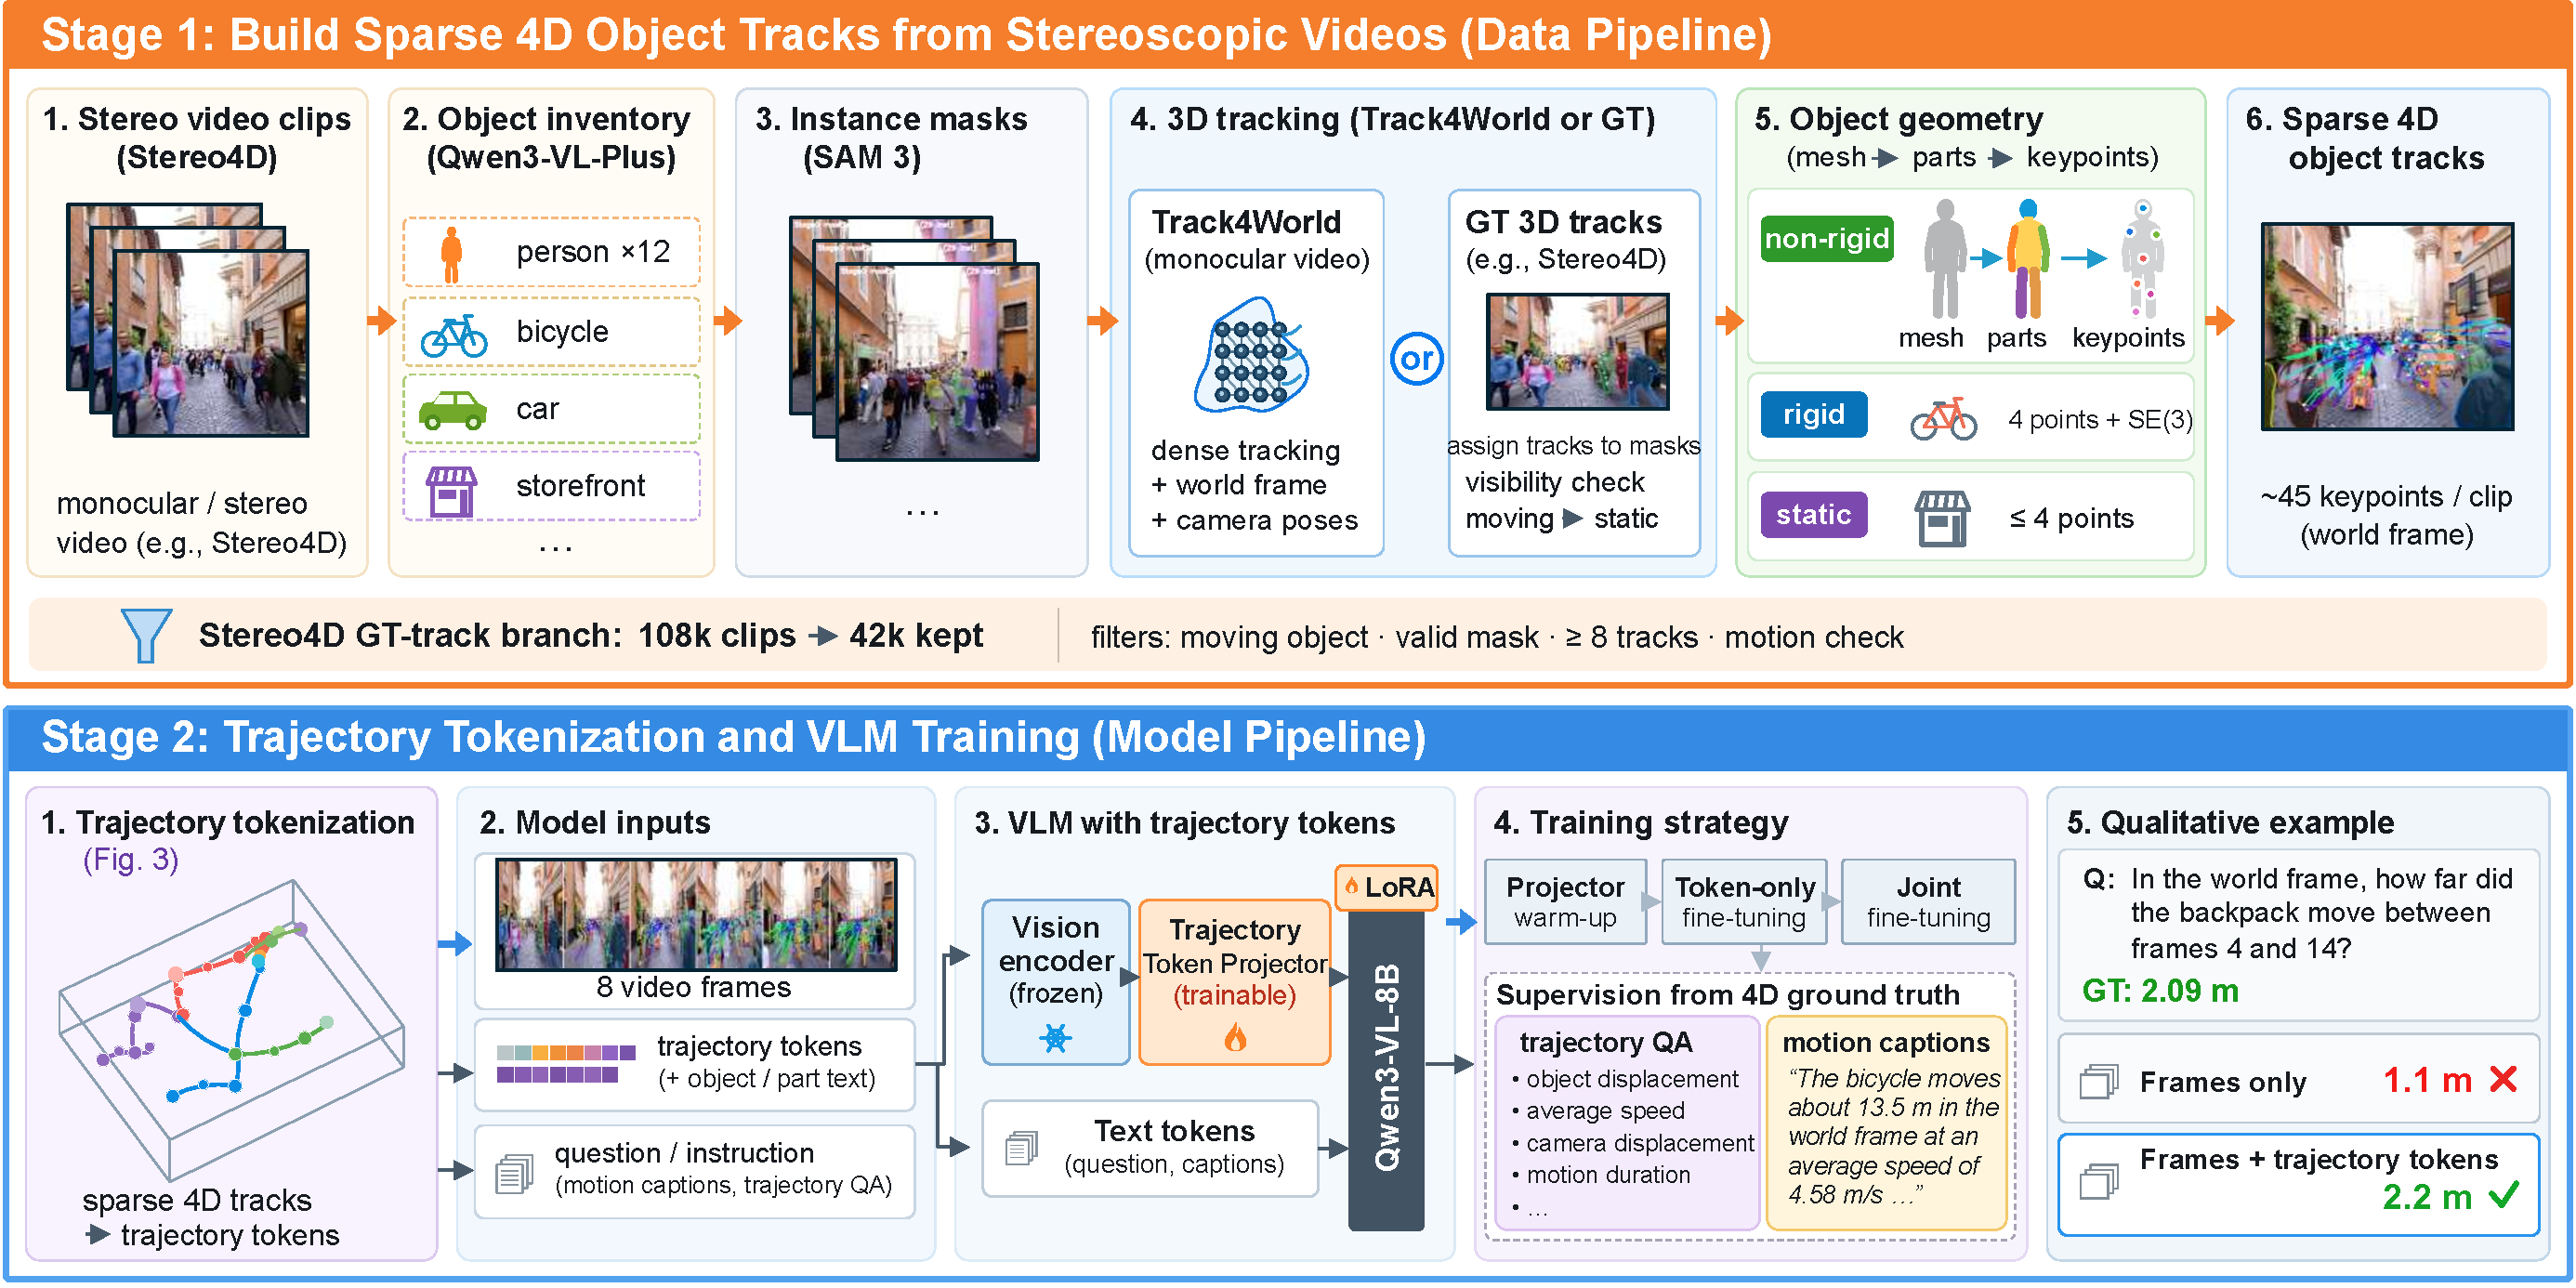
\includegraphics[width=\linewidth]{fig2_pipeline_20260926.pdf}
\caption{\textbf{Pipeline with real video frames and reconstructed tracks.} The upper row implements the Object-Centric Track Constructor; the lower row links the Event-Aware Trajectory Tokenizer to the Trajectory-Language Adapter and its three training stages. The reported QA uses released Stereo4D tracks. In the supplied artwork, ``GT'' means released reconstructed tracks, ``ground truth'' means reconstruction-derived references, and ``average speed'' means endpoint displacement rate. Track4World is an optional branch not used in the reported QA.}
\label{fig:pipeline}
\end{figure}

% ----------------------------------------------------------------------
\subsection{Object-Centric Track Constructor}
\label{sec:repr}

Figure~\ref{fig:pipeline} (top) summarizes how a video clip is converted into
\emph{sparse 4D object tracks}.
We first obtain per-object masks and dense 3D tracks with visibility and camera poses. All reported TrajQA-B results use Stereo4D's released tracks; Track4World~\citep{luTrack4WorldFeedforwardWorldcentric2026} is an optional path for other monocular videos that is not evaluated in the downstream QA results. For non-rigid objects, SAM 3D Objects~\citep{sam3dteam2025sam3d3dfyimages} reconstructs an object mesh that is partitioned into semantic parts by PartSAM~\citep{zhuPartSAMScalablePromptable2026};
representative surface keypoints are then selected and associated with the corresponding dense tracks. The complete extraction pipeline, including object discovery with Qwen3-VL-Plus,
mask propagation with SAM~3~\citep{ICLR2026_e0982cbc}, mesh reconstruction, and keypoint sampling and association, is detailed in Appendix~\ref{app:pipeline}.

The resulting representation is object-centric, part-aware, and metric. A non-rigid object uses sparse keypoints assigned to semantic parts; a rigid object uses four reference keypoints and a per-frame pose $(\mR_i,\vt_i)\in SE(3)$ estimated from its tracks; and a static object uses up to four points. For object $o$ with $K_o$ keypoints, the module returns positions $\tX_o\in\R^{K_o\times T\times 3}$, visibility $\mV_o\in\{0,1\}^{K_o\times T}$, a part index for each keypoint, and a text label. Here $T$ is the number of frames, $\mR_i\in SO(3)$ is a rigid rotation, and $\vt_i\in\R^3$ is its translation. Camera poses and timestamps are stored alongside the object tracks. All coordinates are in the reconstructed world frame, so object and camera motion can be distinguished. A scene contains 44.8 selected keypoints on average (20.7 on moving objects), rather than hundreds of dense tracks per object.

% ----------------------------------------------------------------------
\subsection{Event-Aware Trajectory Tokenizer}
\label{sec:token}

\begin{figure}[t]
\centering
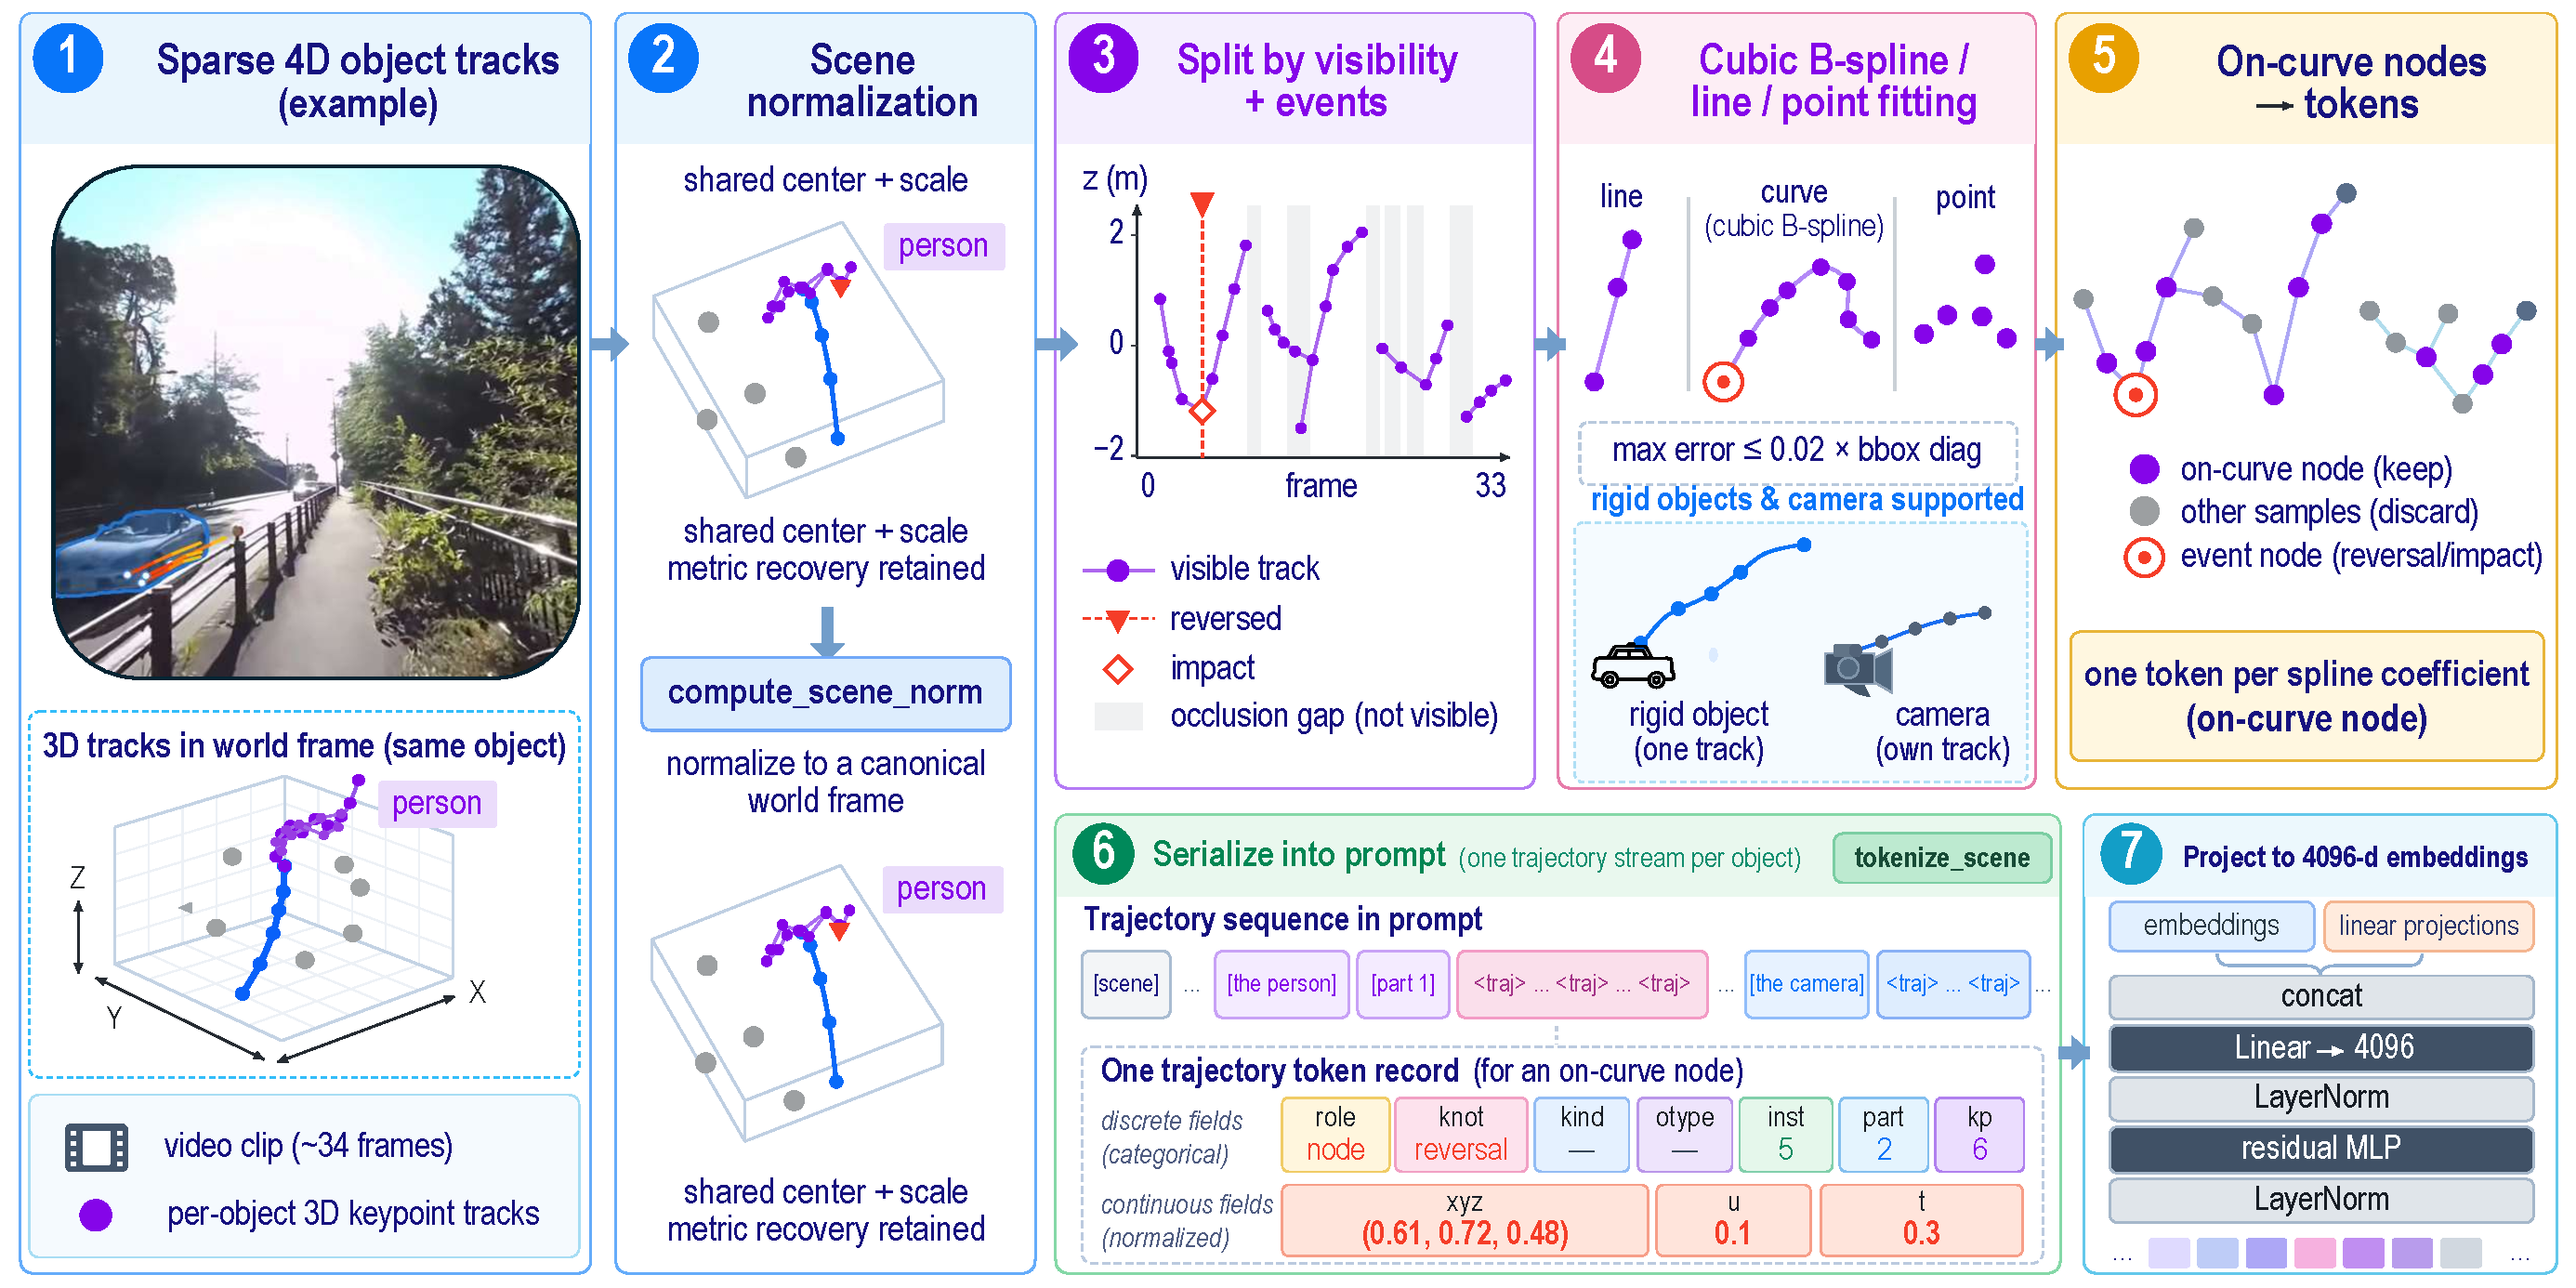
\includegraphics[width=\linewidth]{fig3_tokenization_editable.pdf}
\caption{\textbf{From a keypoint track to trajectory tokens} (one pedestrian keypoint). The scene is normalized; visible runs are split at motion events; spline pieces are fitted with a target error of $0.02$ times the trajectory bounding-box diagonal. Fitted on-curve nodes are serialized by object and part with text labels and projected into the LLM embedding space. A small fraction of pieces cannot meet the target under the node budget (Appendix~\ref{app:tokenization}).}
\label{fig:tokenization}
\end{figure}

\paragraph{Normalization and segmentation.}
All visible keypoints of a scene are shifted by their centroid $\boldsymbol{\mu}\in\R^3$ and scaled by the maximum radius $s>0$ into the unit sphere, $\tilde{\vp}=(\vp-\boldsymbol{\mu})/s$; $(\boldsymbol{\mu},s)$ are emitted as the scene header, so a metric position is recoverable as $\vp=s\tilde{\vp}+\boldsymbol{\mu}$.
A track is fitted only on its maximal visible runs: an occlusion gap is recorded explicitly rather than silently interpolated.
Within a run we detect motion \emph{events} on the inter-frame displacements: a direction change exceeding $90^\circ$ when both steps exceed a noise floor (called a reversal in the token vocabulary), or a peak in discrete acceleration (called an impact). We split the run at these event frames.
Consecutive pieces include the same observed event frame, but separate smoothing fits need not interpolate it exactly. Splitting permits a local change of direction or acceleration that a single global smooth fit might attenuate; its benefit for QA remains to be isolated experimentally.

\paragraph{Target-error fit.}
For observed frames $f_0<\dots<f_{m-1}$, let $u_i=(f_i-f_0)/(f_{m-1}-f_0)$ and fit a cubic B-spline to normalized positions $\tilde{\vp}_i$:
\begin{equation}
\mB(u)=\sum_{h=1}^{n} N_{h,3}(u;\boldsymbol{\xi})\,\boldsymbol{\beta}_h,\qquad
\max_i\|\mB(u_i)-\tilde{\vp}_i\|_2\leq\varepsilon=\alpha d,\quad \alpha=0.02.
\label{eq:fit}
\end{equation}
Here $n\leq12$ is the coefficient count, $N_{h,3}$ is the cubic basis on knot vector $\boldsymbol{\xi}$, $\boldsymbol{\beta}_h\in\R^3$ is a control point, and $d$ is the bounding-box diagonal of the object's normalized visible path. Adaptive knots allocate more nodes to harder motion. The sampled bound holds for 99.82\% of pieces; the rest retain their best fit and are counted as failures (Appendix~\ref{app:tokenization}).

\paragraph{On-curve nodes as tokens.}
For knot values $\xi_l$, the Greville parameter $\tau_h=(\xi_{h+1}+\xi_{h+2}+\xi_{h+3})/3$ yields the on-curve sample $\mB(\tau_h)$, unlike an off-curve spline control point. We serialize one node per coefficient with its mapped physical timestamp and a smooth, event, or endpoint flag. The question generator linearly interpolates these records to obtain a decoded path $\hat{\vp}(t)$ and checks its answers against the references (Gate~0). The LLM does not receive the knot vector, so the fit bound in Eq.~\ref{eq:fit} is not an error bound on $\hat{\vp}(t)$; separate event-side fits may also disagree at their shared time. Appendix~\ref{app:tokenization} details this distinction. Rigid objects fit translation and rotation jointly on shared knots; their keypoints follow $\vp_j(t)=\mR_t\tilde{\vr}_j+\vc(t)$, where $\tilde{\vr}_j\in\R^3$ is a reference point, $\mR_t\in SO(3)$ is rotation, and $\vc(t)\in\R^3$ is translation. The camera is appended as a rigid pseudo-object.

\paragraph{Serialization.}
Each record has seven discrete fields (role, knot type, kind, VLM type, instance, part, keypoint) and three continuous fields (3D value, normalized clip time, absolute seconds). A scene header stores $(\boldsymbol{\mu},s)$; objects follow with text category and part labels adjacent to their trajectory placeholders, and the camera comes last. A clip uses a median of 165 trajectory tokens against 1,152 visual tokens from eight frames. Training caps the stream at 512 records while keeping structural and event nodes.

\subsection{Trajectory-Language Adapter}
\label{sec:train}

\paragraph{Trajectory Token Projector.}
The projector (Fig.~\ref{fig:tokenization}, right) maps every token independently. Let $d_1,\ldots,d_7$ denote its seven discrete field values; $\vx\in\R^3$ is its position, rotation, reference point or gap value, $u\in[0,1]$ is normalized clip time, and $t$ is physical time in seconds. Learned tables $\mE_k$ embed discrete fields, learned matrices $\mW_{\vx},\mW_u,\mW_t$ project continuous fields, and binary gates $g_{\vx},g_u,g_t$ mark fields present in this token. A learned fusion matrix $\mW_{\mathrm f}$ and bias $\vb_{\mathrm f}$ precede layer normalization (LN) and a residual multilayer perceptron (MLP):
\begin{align}
\vh&=\mW_{\mathrm{f}}\big[\mE_1(d_1);\dots;\mE_7(d_7);\;g_{\vx}\mW_{\vx}\vx;\;g_u\mW_u u;\;g_t\mW_t t\big]+\vb_{\mathrm{f}},
\label{eq:projector}\\
\vz&=\mathrm{LN}\big(\vh'+\mathrm{MLP}(\vh')\big),\qquad \vh'=\mathrm{LN}(\vh),\nonumber
\end{align}
with 85.93M parameters in total.
Here $\vh$ is the fused field representation, $\vh'$ its normalized value, and $\vz$ the output token embedding.
It contains no attention, convolution or pooling, so every relation between trajectories is formed inside the LLM.
Its outputs replace the placeholder embeddings by a masked scatter into the LLM's input embeddings; trajectory tokens are otherwise treated as text (ordinary 1-D positions on all rotary axes) and never pass through the vision encoder.

% ----------------------------------------------------------------------

The backbone is Qwen3-VL-8B-Instruct with frozen vision and base weights. We train the projector and language-model LoRA adapters~\citep{huLoRALowRankAdaptation2021} by next-token cross-entropy on generated evidence and answer text. Stage~1 warms up the projector on rule-generated motion captions with the base model frozen; Stage~2 learns token-only QA with the projector and LoRA; Stage~3 restores frames and drops them independently with probability 0.2 while keeping tokens. This sequence first teaches the new interface to express motion and then adapts it to metric questions. All three training stages exclude QA evaluation scenes; stages~2 and~3 additionally use source-video-disjoint QA splits. A stage-1 source-video audit remains to be documented (Appendix~\ref{app:training}).


% ======================================================================
% Experiments (restructured 2026-09-26 around RQ1-RQ3; approved plan).
% Tables 2 and 3 are native LaTeX tables generated from
% paper/trajqa_b_results_20260925_1300/{results_table.md, figure/Ablation.md}
% (identical to the package's PNG tables, cross-checked against the CSVs);
% Table 4 is parsed from TRAJQA_B_SPEC.md §21.8 (held-out block).
% Protocol details, full tables and secondary diagnostics: Appendix app:exp_setup.
% ======================================================================
\section{Experiments}
\label{sec:experiments}

\paragraph{Dataset and evaluation.}
\label{sec:qa}
TrajQA-B draws on 42,151 curated Stereo4D scenes and uses source-video-disjoint QA splits: 56,120 training, 1,318 validation, 4,492 test, and 3,430 additional held-out questions (Table~\ref{tab:qa-splits}). Seven question families cover camera and object displacement, endpoint displacement per elapsed second, interval comparisons, motion source, and duration (Appendix~\ref{app:qa}). The three four-choice numeric families contribute 7,500 evaluation questions and have 25.0\% uniform-guessing accuracy. In every table \emph{speed} means endpoint displacement divided by elapsed time, rather than path length per time. Gate~0 retains questions whose reference answer a deterministic reader can reproduce from the capped records; this tests record reading and calculation, not reconstruction accuracy. Option ranks and binary answers are balanced, then audited against question-only heuristics. The separately selected stage-1 caption training scenes also exclude QA evaluation scenes; its source-video overlap has not been audited (Appendix~\ref{app:training}). Appendix~\ref{app:exp_setup} gives the full protocols and denominators.

\paragraph{Implementation details.}
Our backbone is Qwen3-VL-8B-Instruct with frozen vision and base language weights. The trainable trajectory projector has 85.93M parameters; language-model LoRA adapters have rank 128, scale 256, dropout 0.05, and 349.18M parameters. Each sample contains eight uniformly sampled video frames, resized to a longest side of 384 pixels (144 visual tokens per frame), the object-labelled trajectory stream capped at 512 records, and a question or instruction. We use three stages: 26,000-step projector warm-up on 64,523 rule-generated motion captions from a separately selected caption corpus; 8,400-step projector-plus-LoRA QA training with trajectory tokens but no frames; and 3,507-step joint QA training with frames restored and independently dropped with probability 0.2. All stages use AdamW with $\beta=(0.9,0.95)$, zero weight decay, gradient clipping at 1.0, global batch size 16, and seed 0. The peak projector learning rate is $2\times10^{-4}$ throughout; the adapters use $10^{-4}$ in stages 2 and 3. We train on the assistant's evidence and answer text with next-token cross-entropy and decode greedily. The frames-only Qwen3-VL-8B control was fine-tuned on the same QA training split, although its exact schedule and checkpoint selection are unavailable in the manuscript. Most external baselines are zero-shot and some use their official video pipelines or a smaller proprietary-model subset; they contextualize performance rather than isolate the effect of trajectory input. Stage-1 captions use metadata frame rate while QA targets use frame timestamps, a source of noisy time labels described in Appendix~\ref{app:data_curation}.

% ----------------------------------------------------------------------
\subsection{Comparisons on TrajQA-B}
\label{sec:exp-main}

\begin{table}[t]
\caption{TrajQA-B numeric accuracy (\%). Numeric-3 pools the three four-choice families ($n=7{,}500$; guessing: 25.0); split and family scores are also shown. External models are zero-shot except MLLM-4D-SFT, while ours is fine-tuned on the TrajQA-B training split. Proprietary models use a 1,000-question subset. Bold marks the largest displayed score in each column; protocols and subsets differ. Full results appear in Appendix~\ref{app:exp_setup}.}
\label{tab:main}
\begin{center}
\small
\setlength{\tabcolsep}{3.6pt}
\begin{tabular}{lcccccc}
\toprule
\textbf{Model} & \textbf{Numeric-3}$\uparrow$ & \textbf{Held-out}$\uparrow$ & \textbf{Test}$\uparrow$ & \textbf{Cam.\ disp.}$\uparrow$ & \textbf{Obj.\ disp.}$\uparrow$ & \textbf{Rate}$\uparrow$ \\
\midrule
\rowcolor{blue!12}\multicolumn{7}{l}{\emph{Proprietary models (1,000-question subset)}} \\
GPT-6 Astra & 39.2 & 37.9 & 40.5 & 46.0 & 32.7 & 33.9 \\
Claude Fable 5.1 & 35.2 & 35.8 & 34.5 & 39.6 & 35.2 & 26.9 \\
\midrule
\rowcolor{teal!12}\multicolumn{7}{l}{\emph{Open-source base models, 7B and 8B}} \\
Qwen2.5-VL-7B & 27.3 & 26.6 & 27.9 & 27.1 & 27.7 & 27.3 \\
Qwen3-VL-8B & 28.1 & 28.5 & 27.7 & 28.9 & 27.9 & 26.9 \\
LLaVA-NeXT-Video-7B & 25.0 & 24.5 & 25.4 & 25.7 & 24.2 & 24.7 \\
InternVideo2.5-8B & 25.5 & 25.5 & 25.5 & 25.5 & 24.9 & 26.1 \\
InternVL2.5-8B & 27.0 & 27.3 & 26.8 & 27.7 & 27.4 & 25.5 \\
InternVL3.5-8B & 26.8 & 25.8 & 27.5 & 26.3 & 26.4 & 27.9 \\
\midrule
\rowcolor{teal!12}\multicolumn{7}{l}{\emph{Open-source base models, 32B}} \\
Qwen2.5-VL-32B & 28.4 & 28.3 & 28.5 & 29.7 & 27.3 & 27.5 \\
Qwen3-VL-32B & 27.8 & 27.8 & 27.7 & 27.9 & 25.9 & 29.5 \\
\midrule
\rowcolor{teal!12}\multicolumn{7}{l}{\emph{Open-source base models, 38B}} \\
InternVL2.5-38B & 29.4 & 29.3 & 29.5 & 30.3 & 29.9 & 27.5 \\
InternVL3.5-38B & 28.5 & 28.9 & 28.3 & 29.4 & 27.5 & 28.2 \\
\midrule
\rowcolor{violet!12}\multicolumn{7}{l}{\emph{3D spatial-reasoning models}} \\
VG-LLM (Qwen2.5-VL-7B) & 25.2 & 24.6 & 25.7 & 24.8 & 25.4 & 25.6 \\
VLM-3R (LLaVA-Video-7B) & 26.9 & 26.9 & 27.0 & 27.1 & 27.0 & 26.7 \\
\midrule
\rowcolor{orange!12}\multicolumn{7}{l}{\emph{4D instruction-tuned model (Stereo4D source)}} \\
MLLM-4D-SFT (Qwen3-VL-8B) & 25.0 & 24.7 & 25.3 & 25.3 & 24.9 & 24.8 \\
\midrule
\rowcolor{green!15}\multicolumn{7}{l}{\emph{TrajQA-B fine-tuned model}} \\
Ours (frames + trajectory tokens) & \textbf{82.2} & \textbf{81.7} & \textbf{82.5} & \textbf{89.4} & \textbf{77.6} & \textbf{75.2} \\
\bottomrule
\end{tabular}
\end{center}
\end{table}

Table~\ref{tab:main} places our model next to 15 external baselines. Open-source and specialised 3D models score between 25.0\% and 29.4\% on the pooled numeric questions; the two proprietary models reach 39.2\% and 35.2\% on their smaller subset. Comparisons from 7B to 38B do not show a clear gain from parameter count in this collection of models, although architectures and video protocols also vary.
MLLM-4D-SFT scores 25.0\% after training on a separate 4D QA corpus drawn from the same source videos; 85\% of evaluation clips appear in its SFT data. Its strong option-position preference provides a plausible explanation for the poor transfer to our balanced options (Appendix~\ref{app:exp_setup}).
Our fine-tuned model reaches 82.2\% overall, with 81.7\% on held-out and 82.5\% on test. A frames-only Qwen3-VL-8B arm trained on the same question split reaches 48.3\% (Table~\ref{tab:ablation}). This task-adapted visual reference lacks timestamps and may omit the queried endpoint frames; its undocumented training schedule also prevents a controlled modality comparison.

% ----------------------------------------------------------------------
\subsection{Input Ablation Studies}
\label{sec:exp-ablation}

\begin{table}[t]
\caption{Input interventions on the full evaluation set. All rows except frames only use the same final model; that row uses a separately fine-tuned visual model. Bold marks the best value in each column, including ties. Donor tokens replace trajectory content with that of another scene while preserving format, count, and timestamps. Cam./Obj.: camera/object displacement; rate: endpoint displacement per elapsed second. All results use one training seed.}
\label{tab:ablation}
\begin{center}
\footnotesize
\setlength{\tabcolsep}{3pt}
\begin{tabular}{lcccccccc}
\toprule
\textbf{Inputs at inference} & \textbf{Frames} & \textbf{Tokens} & \textbf{Numeric-3}$\uparrow$ & \textbf{Held-out}$\uparrow$ & \textbf{Test}$\uparrow$ & \textbf{Cam.}$\uparrow$ & \textbf{Obj.}$\uparrow$ & \textbf{Rate}$\uparrow$ \\
\midrule
Question only & No & No & 26.8 & 27.5 & 26.2 & 27.2 & 27.0 & 25.9 \\
Frames only (separate FT) & \checkmark & No & 48.3 & 47.8 & 48.8 & 53.7 & 44.5 & 43.9 \\
Frames + donor tokens & \checkmark & donor & 29.6 & 30.6 & 28.8 & 30.7 & 28.8 & 28.6 \\
Trajectory tokens only & No & \checkmark & \textbf{82.2} & 81.5 & \textbf{82.8} & \textbf{89.4} & \textbf{77.7} & \textbf{75.5} \\
Frames + traj.\ tokens (full) & \checkmark & \checkmark & \textbf{82.2} & \textbf{81.7} & 82.5 & \textbf{89.4} & 77.6 & 75.2 \\
\bottomrule
\end{tabular}
\end{center}
\end{table}

\begin{table}[t]
\caption{Metric grounding of generated evidence on held-out numeric questions ($n=3{,}312$). Acc.: accuracy; $E_{\mathrm{obj}}$ / $E_{\mathrm{cam}}$: median position error. Bold marks the best value for each metric, including ties. Within $1.2\times$: fraction whose stated camera displacement / object displacement / endpoint rate differs from the reference by less than a multiplicative factor of 1.2.}
\label{tab:evidence}
\begin{center}
\footnotesize
\setlength{\tabcolsep}{3pt}
\begin{tabular}{lcccc}
\toprule
\textbf{Inputs at inference} & \textbf{Acc.}$\uparrow$ & $\boldsymbol{E_{\mathrm{obj}}}$ \textbf{(m)}$\downarrow$ & $\boldsymbol{E_{\mathrm{cam}}}$ \textbf{(m)}$\downarrow$ & \textbf{Within $1.2\times$ $\uparrow$: cam / obj / rate} \\
\midrule
Question only & 27.5 & 3.56 & 0.83 & 21.0 / 15.5 / 14.9 \\
Frames + donor tokens & 30.6 & 3.44 & 1.35 & 18.2 / 17.7 / 16.0 \\
Trajectory tokens only & 81.5 & \textbf{0.32} & \textbf{0.14} & \textbf{91.4} / \textbf{80.0} / \textbf{80.3} \\
Frames + trajectory tokens (full) & \textbf{81.7} & 0.33 & \textbf{0.14} & 91.1 / \textbf{80.0} / 79.9 \\
\bottomrule
\end{tabular}
\end{center}
\end{table}

\textbf{Trajectory content changes the answers.}
The same final model scores 26.8\% with the question alone and 29.6\% with frames plus another scene's tokens, versus 82.2\% with the correct tokens (Table~\ref{tab:ablation}). Both controls remain above uniform guessing, so they do not establish the complete absence of shortcuts; their large gap from the correct-token condition shows that trajectory content matters. The separately trained frames-only arm reaches 48.3\%, roughly 34 points below the full model. On held-out questions, the donor-token intervention lowers accuracy from 81.7\% to 30.6\%. The final model without frames also scores 82.2\% (Appendix~\ref{app:exp_setup}), indicating that this benchmark mainly probes use of supplied metric tracks rather than added value from fusing frames with them.

\textbf{Generated evidence tracks metric quantities.}
On held-out questions, the positions stated in the model's evidence differ from the reference by a median of 0.33~m for objects and 0.14~m for the camera (Table~\ref{tab:evidence}). Its stated displacement or speed lies within a factor of 1.2 of the reference on 80\% to 91\% of questions. With donor tokens, median position errors rise to metres and these rates fall to 16\% to 18\%. The evidence analysis supports use of the trajectory values beyond selecting an option, subject to the reference-track quality and parsing protocol in Appendix~\ref{app:exp_setup}. Qualitative examples appear in Appendix~\ref{app:qualitative}.

\textbf{Module-facing diagnostics.}
Selected scenes average 44.8 keypoints; the tokenizer uses a median of 165 records and its intermediate spline fits meet the target on 99.82\% of pieces. Donor substitution probes use of correct records. All three main numeric families can be answered from endpoint positions and times, so these diagnostics do not establish a benefit from part labels, event splitting, adaptive fitting, or projector warm-up.

\textbf{Where the improvement applies.}
Camera displacement is the easiest numeric family for the full model (89.4\%), followed by object displacement (77.6\%) and endpoint rate (75.2\%). The final model has the same pooled score with tokens alone as with tokens and frames (82.2\%), so these results demonstrate use of reconstructed motion, not added value from visual fusion. The 81.7\% held-out and 82.5\% test scores show similar performance across the two QA splits, but stage-1 source-video overlap has not been audited. Because donor input remains above 25\% chance and the visual arm lacks queried timestamps, neither control rules out all shortcuts or supplies a fully matched visual comparison.

\paragraph{Evaluation composition.}
Table~\ref{tab:qa-splits} shows the family denominators and the number of scenes and source videos in each split. The held-out and test splits contain 3,292 camera-displacement, 2,172 object-displacement, and 2,036 endpoint-rate questions; these are the 7,500 questions underlying the pooled numeric score. The other four families contribute 422 evaluation questions in total. Their reported aggregate in Appendix~\ref{app:exp_setup} is therefore a smaller, heterogeneous diagnostic, not evidence that the proposed event and part representations improve interior-motion reasoning.

\begin{table}[H]
\caption{TrajQA-B split counts (descriptive, not performance metrics). Splits are disjoint in source videos. Cam./Obj./Rate count the three 4-way families (chance 25\%); Other pools interval\_disp, interval\_speed, motion\_source, and binary motion\_duration. Rate denotes endpoint displacement divided by elapsed time.}
\label{tab:qa-splits}
\begin{center}
\footnotesize
\setlength{\tabcolsep}{3pt}
\begin{tabular}{lrrrrrrr}
\toprule
\textbf{Split} & \textbf{Questions} & \textbf{Cam.} & \textbf{Obj.} & \textbf{Rate} & \textbf{Other} & \textbf{Scenes} & \textbf{Videos} \\
\midrule
train & 56,120 & 21,240 & 16,492 & 14,980 & 3,408 & 12,409 & 2,198 \\
validation & 1,318 & 524 & 404 & 340 & 50 & 668 & 162 \\
dev test & 4,492 & 1,692 & 1,284 & 1,212 & 304 & 2,241 & 578 \\
held-out test & 3,430 & 1,600 & 888 & 824 & 118 & 862 & 166 \\
\bottomrule
\end{tabular}
\end{center}
\end{table}

\noindent\textbf{Residual data risks.}
Because 98.4\% of clips share a source video, the unaudited stage-1 source-video intersection remains consequential. Caption frame rates differ from QA timestamps by more than 10\% in 12.85\% of scenes, potentially adding rate-label noise.


\section{Conclusion}
\label{sec:conclusion}
Sparse Trajectory Tokens turn reconstructed tracks into compact metric records for an MLLM. TrajQA-B accuracy is 82.2\% with correct records and 29.6\% with donor records; a separate frames-only reference scores 48.3\%. Token-only accuracy is also 82.2\%, so frames add no measured benefit here. Endpoint questions cannot isolate tokenization components. Generalization to unseen source videos, component effects, and physical validity need a stage-1 source-video audit, matched visual inputs, ablations, and independent ground truth.

\clearpage
\subsection*{AI Use Statement}
% Required by ICLR 2027; does not count toward the page limit.

Generative AI tools were used solely for grammar correction and minor language polishing of text written by the authors. No generative AI tools were used for any research tasks requiring disclosure under the ICLR 2027 AI Policy. All AI-assisted edits were reviewed by the authors, who take full responsibility for the final content of this work.

\subsection*{Reproducibility statement}
The appendix describes the data source, QA split rule, curation gates, token
fields, spline fitting, question generator, and trajectory-model schedules.
Exact reproduction additionally requires the Stereo4D reconstructions,
training and evaluation code, model checkpoints, the frames-only training
recipe, and the donor-token mapping; the latter two are not documented in the
available manuscript. Reported trained-model results use one seed.

\subsection*{Ethics statement}
The source videos may include identifiable people. Our analysis uses the
Stereo4D reconstructions and selected illustrative frames; any redistribution
of videos or derived visual assets should follow the source permissions and
applicable privacy requirements. Automatic curation favors objects that can be
segmented and tracked reliably, so the retained scenes should not be treated
as a representative sample of all activities or environments.

\bibliography{iclr2027_conference}
\bibliographystyle{iclr2027_conference}

\appendix
% ======================================================================
% Appendix (2026-09-25): implementation, dataset-construction and
% reproducibility details moved out of the Method section.  Every number
% was verified against the repository on 2026-09-25 (see the header of
% sections/method.tex.v1_long for the source files).
% ======================================================================

\section{Data Curation Details}
\label{app:data_curation}

\paragraph{Source data and frame sampling.}
The official Stereo4D index lists 108,015 clips; 3D tracks are released for 89,454 of them, which form our candidate pool.
Every clip is decoded from the rectified left view at $512\times512$ pixels and temporally subsampled from the native 30~fps with a per-clip stride $\sigma=\min\!\big(\max(1,\lfloor (N-1)/19\rfloor),\,6\big)$, where $N$ is the number of source frames, so that a clip keeps 20--34 frames (up to 38 are accepted) at an effective rate of $30/\sigma$~fps.
Over the delivered scenes, 76.9\% use stride~6 (5~fps); the frame count ranges from 20 to 38 with a median of 34, and 67.6\% of the scenes have exactly 34 frames.
The per-frame timestamps of the release are kept with every scene. Trajectory tokens and QA targets use these timestamps; stage-1 motion captions instead use the metadata frame rate. The two time sources disagree by more than 10\% in 12.85\% of scenes, which introduces noise into time-dependent caption targets.

\paragraph{Curation steps.}
A clip enters the training set only if at least one object moves in the world frame and this motion is observable both in the released tracks and in the image.
The steps, and the number of clips each removes, are (the funnel in Fig.~\ref{fig:pipeline} summarizes them as 108k $\rightarrow$ 42k):
\begin{itemize}
\item \emph{Object inventory.} A VLM (Qwen3-VL-Plus) inspects 8 uniformly spaced frames and returns, for every object, a category label, a 2D box on one frame, a rigid/non-rigid attribute and a static/dynamic attribute; the prompt asks it to discount camera motion. Clips in which every object is static are discarded before any further processing (29,915).
\item \emph{Instance masks.} SAM~3 is prompted with each label and its box on the VLM's frame (text-only retry on failure) and propagates the mask bidirectionally through the clip. Masklets whose largest single-frame area is below 0.3\% of the image are dropped, and masklets of different concepts with temporal IoU above 0.5 are merged. Clips in which no dynamic object obtains a mask are discarded (9,207, of which 1,292 receive no mask at all).
\item \emph{Track attribution.} Every released 3D track is projected into the frames and attributed to the instance whose mask (dilated by 4~px) contains at least 50\% of its visible projections and beats the runner-up by a margin of 0.15; only tracks visible in at least 3 frames are eligible, and at most 800 tracks per instance are kept by farthest-point sampling. A dynamic instance is kept only if it owns at least 8 tracks (4 for a static instance), one of which falls on its undilated mask. Clips whose dynamic objects all fail this test are discarded (5,725).
\item \emph{Motion check.} A one-way gate demotes a dynamic instance to static when the median world-frame speed of its tracks is below 0.05~m/s and a static 3D point explains its tracks up to a median image residual of 1~px; it never promotes a static instance. Clips whose last dynamic object is demoted are discarded (2,444).
\item \emph{Failures.} 11 clips failed (7 rejected by the VLM API's content filter, 4 pipeline give-ups).
\end{itemize}

\paragraph{Outcome and splits.}
The remaining 42,152 clips come from 4,079 source videos; one clip with a corrupt reconstruction file is excluded from QA generation, leaving 42,151 QA scenes with, on average, 9.9 objects and 44.8 keypoints per scene (20.7 on moving objects).
Since a source video contributes several clips (median 5, up to 160; 98.4\% of the clips share their video with at least one other clip), the QA splits are made by hashing source-video id. The separate stage-1 caption training selection excludes QA evaluation scenes; its source-video-level relation to the QA splits is not documented here.
The pipeline's numerical gates check consistency among attributed tracks, projected motion, and serialized answers. They do not provide an independent measurement of metric reconstruction fidelity or a human audit of object identity and mask correctness. Errors in either upstream stage can therefore survive a token-side answer check.

% ----------------------------------------------------------------------
\section{Trajectory Representation Pipeline Details}
\label{app:pipeline}

\paragraph{Tracking module.}
Two interchangeable implementations produce the same output, namely per-object dense 3D tracks with per-frame visibility, together with camera poses.
(i)~For ordinary monocular video we use Track4World: a dense grid of query points is seeded inside every instance mask (about 200 seeds per object, at most 2,000 tracks), tracked in a few shared passes with the first camera as world frame, and re-tracked once more at the reference frame $t^\ast$ after the mesh is available.
(ii)~For datasets that release 3D tracks we use the released tracks, attributed to instances as in Appendix~\ref{app:data_curation}.
All Stereo4D scenes in this paper use (ii); none of our training trajectories comes from a learned tracker.

\paragraph{Tracker selection.}
We selected Track4World after a bake-off of five 3D trackers on three datasets (Table~\ref{tab:bakeoff}): DAVIS (no 3D ground truth; only the fraction of tracked points that stay on the object mask is measured), MOVi and PointOdyssey (3D ground truth).
Evaluation points were unified across trackers and queries were released at the same frames.
Track4World has the highest DAVIS on-mask score and the best EPE-2D, $\delta_8$, and OA values on MOVi and PointOdyssey in this table. Other methods obtain the lowest EPE-3D on those two datasets, so the choice reflects the tracking and visibility metrics used by the pipeline rather than a uniform win across metrics.
% Source: EXPERIMENTS_ARCHIVE.md §1 (scoreboard EXPERIMENTS_ARCHIVE/bakeoff2/scoreboard.json).  The re-lock
% rate at 20 frames is omitted from the table: on MOVi it rests on single-digit sample counts.

\begin{table}[t]
\caption{Tracker bake-off (five trackers, three datasets). EPE-2D is measured in pixels and EPE-3D in each dataset's 3D coordinate units (lower is better); $\delta_8$ is the fraction of points within 8~px, OA is occlusion accuracy, and on-mask is the fraction of tracked points remaining on the object mask (higher is better). Bold marks the best available value for each dataset and metric.}
\label{tab:bakeoff}
\begin{center}
\footnotesize
\setlength{\tabcolsep}{3pt}
\begin{tabular}{llrrrrr}
\toprule
\textbf{Tracker} & \textbf{Dataset} & \textbf{EPE-2D}$\downarrow$ & $\boldsymbol{\delta_8}\uparrow$ & \textbf{OA}$\uparrow$ & \textbf{EPE-3D}$\downarrow$ & \textbf{on-mask}$\uparrow$ \\
\midrule
Track4World & DAVIS & -- & -- & -- & -- & \textbf{0.9155} \\
 & MOVi & \textbf{1.722} & \textbf{0.9257} & \textbf{0.8778} & 0.3532 & -- \\
 & PointOdyssey & \textbf{10.410} & \textbf{0.5597} & \textbf{0.8296} & 0.3087 & -- \\
\midrule
TAPIP3D~\citep{zhangTAPIP3DTrackingAny2025} & DAVIS & -- & -- & -- & -- & 0.9032 \\
 & MOVi & 1.836 & 0.9124 & 0.8599 & 0.4259 & -- \\
 & PointOdyssey & 23.462 & 0.3647 & 0.7182 & 0.6936 & -- \\
\midrule
SpaTrackerV2~\citep{xiaoSpatialTrackerV23DPoint2025} & DAVIS & -- & -- & -- & -- & 0.8970 \\
 & MOVi & 1.918 & 0.9043 & 0.8576 & 0.4908 & -- \\
 & PointOdyssey & 16.937 & 0.4130 & 0.7795 & \textbf{0.3029} & -- \\
\midrule
4RC~\citep{luo4RC4DReconstruction2026} & DAVIS & -- & -- & -- & -- & 0.7417 \\
 & MOVi & 2.031 & 0.9066 & 0.8541 & \textbf{0.2653} & -- \\
 & PointOdyssey & 100.364 & 0.3320 & 0.3931 & 0.3546 & -- \\
\midrule
D4RT~\citep{zhangEfficientlyReconstructingDynamic2025} & DAVIS & -- & -- & -- & -- & 0.5898 \\
 & MOVi & 2.852 & 0.8583 & 0.8480 & 0.3695 & -- \\
 & PointOdyssey & 234.402 & 0.0031 & 0.7304 & 1.6874 & -- \\
\bottomrule
\end{tabular}
\end{center}
\end{table}

\paragraph{Object geometry and keypoints.}
Objects are routed by type.
\emph{Non-rigid dynamic} objects are reconstructed with SAM 3D Objects (Fast-SAM3D implementation~\citep{fengFastSAM3D3DfyAnything2026}) from the best of at most three candidate reference frames (chosen by mask agreement), segmented into semantic parts with PartSAM (fragments are merged into neighbouring parts), and sampled on the mesh surface in two passes: the first draws farthest-point, curvature-weighted vertices per part until a coverage of 0.10 part diagonals is reached (at most 64 per part); the second keeps one medoid keypoint per semantic part among candidates that are visible in at least half of the frames, and discards points that are never observed.
\emph{Rigid dynamic} objects skip the mesh when the VLM calls them rigid, a conservative rigidity test on their raw tracks agrees, and they are present in a single contiguous segment; they receive 4 farthest-point keypoints and a per-frame pose $(\mR_t,\vt_t)\in SE(3)$ obtained by Kabsch alignment over all tracked keypoints (the pose is marked undefined when fewer than $\max(3,0.1T)$ frames are solved or the reconstruction residual exceeds one bounding-box extent).
\emph{Static} objects keep 4 representative points (farthest-point sampling of per-track median positions) and no mesh.

\paragraph{Keypoint--pixel--track linking.}
At the reference frame $t^\ast$ the track coordinate frame is aligned to the mesh by a Umeyama similarity; every keypoint is projected into the image and linked to the dense track that passes through that pixel; keypoints occluded at $t^\ast$ are placed by the SE(3) motion of their part before linking.
Each keypoint thereby inherits one metric 3D track over the whole clip together with its per-frame visibility.
The pipeline output for static objects consists of their representative points only.

% ----------------------------------------------------------------------
\section{Tokenization and Projector Details}
\label{app:tokenization}

Throughout, $T$ is the number of frames of the scene and $d$ the diagonal of the trajectory AABB enclosing an object's visible normalized points across time; $d$ includes motion extent and is not necessarily the object's physical size.

\paragraph{Scene normalization.}
All visible keypoint positions of a scene are shifted by their centroid $\boldsymbol{\mu}$ and scaled isotropically by the maximum radius $s$, $\tilde{\vp}=(\vp-\boldsymbol{\mu})/s$, so that the scene lies in the unit sphere; $(\boldsymbol{\mu},s)$ are emitted in the scene header (for the clip in Fig.~\ref{fig:tokenization}, $\boldsymbol{\mu}=(1.46,2.12,10.06)$~m and $s=10.23$~m).
A low-motion check re-labels a dynamic object as static when its world-frame motion is at most 5~cm and its reprojection shows no image motion (residual below 1~px).

\paragraph{Event detection.}
Inside a visible run we detect two kinds of events on the inter-frame displacements $\vDelta_t=\tilde{\vp}_{t+1}-\tilde{\vp}_t$: a \emph{reversal} at frame $t$ if
$\langle\vDelta_{t-1},\vDelta_t\rangle<0$ and $\|\vDelta_{t-1}\|,\|\vDelta_t\|>\delta$ with the noise floor $\delta=\max\big(0.02\,d,\;0.1\,\mathrm{median}_{t:\|\vDelta_t\|>0}\|\vDelta_t\|\big)$, and an \emph{impact} at $t$ if the second difference $a_t=\|\tilde{\vp}_{t+1}-2\tilde{\vp}_t+\tilde{\vp}_{t-1}\|$ is a local maximum exceeding $\max(\mu_a+2\sigma_a,\,0.05\,d)$.
The run is split at every event frame; adjacent events are not merged.

\paragraph{Fitting procedure.}
We use FITPACK's smoothing spline (\texttt{splprep}) and bisect its smoothing factor (30 iterations) to the largest value that satisfies the target bound in Eq.~\ref{eq:fit}; adaptive knots concentrate nodes on motion that is harder to fit.
A piece may use at most $n=12$ coefficients; if the bound cannot be met within this budget the best fit is kept and counted as a bound failure in preprocessing (3,088 of the 1,729,834 pieces in our data, 0.18\%). No dedicated fit-status field is serialized to the model.
Pieces with fewer than five frames use the lowest degree that meets the bound (a line with 2 coefficients, else a quadratic with 3, else interpolation of all points), and a piece with a single frame is one point.
During preprocessing, the control points can be recovered numerically from the Greville nodes and the fitted knot vector to $10^{-12}$. The LLM receives the node records, not that knot vector; Gate~0 therefore recomputes targets by interpolating the serialized nodes rather than relying on exact spline reconstruction.
Knot-type flags are assigned as follows: \emph{endpoint} for the first and last node of a run, \emph{reversal} or \emph{impact} for the two event-side boundary nodes, and \emph{smooth} otherwise. Since fits are smoothed separately, event-side node positions are not guaranteed to coincide exactly.

\paragraph{What the fit bound measures.}
Let $\hat{\vp}(t)$ denote the piecewise-linear path decoded from the serialized nodes after the record cap. Eq.~\ref{eq:fit} controls the fitted spline at observed frames, whereas the model and Gate~0 use $\hat{\vp}(t)$. Because the knot vector is omitted, that bound does not imply an equal bound for the decoded path. Gate~0 only verifies that the decoded answer remains in the same option cell (or gives the same categorical answer), which is weaker than bounding trajectory error. Each of the three principal numeric questions is determined by two decoded endpoint positions and their timestamps; consequently, these questions do not by themselves test whether interior event nodes, part labels, or adaptive sampling are needed. At a split event, the two fitted sides can produce distinct samples at the same time; the available manuscript does not specify the implementation's duplicate-time interpolation rule or report decoded-path error statistics. These details require a code-level audit before asserting a stronger fidelity guarantee.

\paragraph{Rigid objects and the camera.}
A rigid object is described by its keypoints' reconstruction $\vp_j(t)=\mR_t\,\tilde{\vr}_j+\vc(t)$, where $\tilde{\vr}_j$ are its reference points relative to their centroid and $\vc(t)$ is the normalized centroid trajectory.
Per run we fit the translation $\vc(u)$ and the rotation $\vphi(u)=\log(\mR_{f_0}^{\top}\mR(u))$ (rotation vector relative to the first frame of the run, unwrapped modulo $2\pi$) jointly as one 6-D curve $[\vc(u),\,\rho\,\vphi(u)]$ with shared knots, where $\rho=\max_j\|\tilde{\vr}_j\|$ converts radians into length, and the error bound of Eq.~\ref{eq:fit} is evaluated on the reconstructed keypoints, $\max_{i,j}\|\mR_{f_0}\exp(\vphi(u_i))\,\tilde{\vr}_j+\vc(u_i)-\tilde{\vp}_j(f_i)\|\le\varepsilon$.
Rotation nodes are serialized as absolute rotation vectors.
The camera is encoded as a rigid pseudo-object appended last, whose translation stream is the optical centre (error bound $\min(\varepsilon,\,0.10\text{ m}/s_{\mathrm{norm}})$ in normalized coordinates, at most 48 coefficients). Here $s_{\mathrm{norm}}=s$ is the scene normalization radius in metres, not elapsed seconds.

\paragraph{Token record.}
Every token is a record with seven discrete and three continuous fields (Table~\ref{tab:token-fields}); fields that do not apply to a role are masked by a presence flag.
Besides the node tokens there are structural tokens: three scene-header tokens (frame count and clip duration; normalization centre; normalization scale), one object-header token per object (kind, VLM type, instance index, number of parts, and for rigid objects the SE(3) reconstruction residual), up to four point tokens per static object, the reference-point tokens of rigid objects, and, per non-rigid keypoint, one visibility-summary token and one token per occlusion gap.

\begin{table}[t]
\caption{Fields of a trajectory token. Discrete fields are embedded and continuous fields are projected by the adapter in Sec.~\ref{sec:train}. Declared cardinalities include reserved and padding values beyond the semantic values listed; this table defines fields rather than performance metrics.}
\label{tab:token-fields}
\begin{center}
\small
\begin{tabular}{llp{7.3cm}}
\toprule
\textbf{Field} & \textbf{Type} & \textbf{Values} \\
\midrule
role & discrete (12) & scene header, normalization centre, normalization scale, object header, static point, rigid reference point, rotation node, translation node, keypoint node, occlusion gap, visibility summary \\
knot type & discrete (5) & smooth, reversal, impact, endpoint \\
kind & discrete (4) & static, rigid, non-rigid \\
object type & discrete (4) & rigid, non-rigid (VLM attribute) \\
instance & discrete (65) & per-scene object index \\
part & discrete (17) & semantic part index within the object \\
keypoint & discrete (129) & keypoint index within the part \\
\midrule
xyz & continuous (3) & normalized position, rotation vector, reference point, or gap interval \\
$u$ & continuous (1) & normalized time in the clip, $u=f/(T-1)$ \\
$t$ & continuous (1) & absolute time in seconds from the frame timestamps \\
\bottomrule
\end{tabular}
\end{center}
\end{table}

\paragraph{Serialization and budget.}
The tokens of a scene are serialized as one sequence: the scene header, then every object in order, and the camera last.
Each object is introduced by its category label as ordinary text, followed by its object-header token; a non-rigid object nests its parts as \texttt{[part 1]}, \texttt{[part 2]}, \dots, each followed by the tokens of that part's keypoints (visibility summary, gaps, nodes); a rigid object lists its reference points, rotation nodes and translation nodes; a static object its points.
Several instances of the same category share the same text label, and their identity is carried by the instance field.
Over the 42,151 scenes a clip has a median of 165 trajectory tokens (mean 231, 90th percentile 507, maximum 2,227); for comparison, the 8 video frames occupy 1,152 visual tokens.
At training time a sample is capped at 512 trajectory tokens by keeping all structural tokens and all reversal/impact nodes and thinning the remaining nodes uniformly.

\paragraph{Projector dimensions and injection.}
In Eq.~\ref{eq:projector} every embedding table $\mE_k$ and every linear map $\mW_{\vx},\mW_u,\mW_t$ has 456 output dimensions, so the concatenation has $10\times456=4{,}560$ dimensions; $\mW_{\mathrm{f}}\in\R^{4096\times4560}$ maps it to the LLM dimension $D=4096$, and the MLP is $4096\to8192\to4096$ with GELU.
The output replaces the embedding of the corresponding \texttt{<|traj\_pad|>} placeholder by a masked scatter into the LLM's input embeddings, before the visual tokens are inserted.
The final LayerNorm sets the norm of every injected vector to $\sqrt{D}=64$.

% ----------------------------------------------------------------------
\section{Question Generation Details}
\label{app:qa}

\begin{table}[t]
\caption{Question families and complete numeric grid parameters for TrajQA-B (descriptive table; no performance metric). Numeric families are 4-way with options taken from a fixed logarithmic grid $v_k=v_0\,r^{k}$ ($r=1.35$); the remaining families are 2-way. The internal name speed\_grid denotes endpoint displacement rate. Numeric questions specify frame indices without stating the elapsed time; the duration family instead specifies a time threshold.}
\label{tab:qa-families}
\begin{center}
\footnotesize
\setlength{\tabcolsep}{4pt}
\begin{tabular}{lp{5.6cm}lc}
\toprule
\textbf{Family} & \textbf{Asks for} & \textbf{Options} & \textbf{Needs time?} \\
\midrule
disp\_grid & world-frame displacement of an object in $[i,j]$ (m) & grid, $v_0=0.5$, 12 cells & no \\
speed\_grid & endpoint displacement rate of an object in $[i,j]$ (m/s) & grid, $v_0=0.1$, 14 cells & yes \\
cam\_disp\_grid & displacement of the camera in $[i,j]$ (m) & grid, $v_0=0.5$, 13 cells & no \\
interval\_disp & which of two adjacent intervals covers the longer distance & 2-way & no \\
interval\_speed & which interval has greater endpoint displacement rate & 2-way & yes \\
motion\_source & whether the screen motion is due to the object or the camera & 2-way & no \\
motion\_duration & whether the object keeps moving for more than $X$ seconds & yes/no & yes \\
\bottomrule
\end{tabular}
\end{center}
\end{table}

\paragraph{Reference quantities and observability guards.}
The object position at frame $t$ is the per-frame median of its visible keypoints (for rigid objects the pose applied to the reference points), i.e.\ the same quantity the tokens encode; the camera position is the optical centre from the released poses.
Displacement is the Euclidean distance between the positions at frames $i$ and $j$; the benchmark's ``speed'' target divides this endpoint displacement by elapsed time (intervals shorter than 0.5~s are excluded). It is the magnitude of average velocity, not path length divided by time. Motion duration is the longest contiguous span in which the per-frame speed exceeds 0.05~m/s and the object moves by at least 10~px in a frozen-camera projection.
Windows are random pairs of visible frames with $j-i\ge3$; the two intervals of the comparison families are adjacent, with equal length for interval\_disp and a length ratio of at least 1.5 for interval\_speed, and their displacements (speeds) must differ by a factor of at least 1.4.
A question is generated only if the asked quantity is observable: the displacement must exceed $\max(0.5\text{ m},\,3\,\eta(z))$, where $\eta(z)$ is a depth-dependent noise level of the stereo reconstruction (0.05~m below 5~m, 0.25~m below 10~m, 0.53~m below 20~m, 0.90~m below 40~m; objects beyond 40~m are excluded); the object must move by at least 10~px under a frozen camera; the keypoint-based displacement must agree with the displacement of the object's dense tracks within $\max(0.3\text{ m},0.3\,d)$; radial motion must be corroborated by the change of apparent size; and speeds above 6~m/s for humans (30~m/s otherwise) are rejected.
For motion\_source, the ``camera'' side uses only static objects of movable categories (humans, vehicles, animals) under a camera that moves by at least 0.5~m or 5$^\circ$, and the ``object'' side only dynamic objects under a camera that moves by at most 0.10~m and 1$^\circ$; both require at least 40~px of screen motion.
An object is referred to by its label when it is unique in the scene, or as ``the left/right \emph{label}'' when exactly two instances are separated horizontally by at least 15\% of the image width in every frame the question involves.

\paragraph{Options and balancing.}
Numeric options are the geometric centres of four \emph{adjacent} cells of a fixed global logarithmic grid, $v_0 r^{w+k+0.5}$ for $k=0,\dots,3$, chosen so that the cell of the true value is one of the four; the four letters are randomly permuted, and true values that fall within 6\% of a cell edge are discarded.
The grid is global rather than adapted to a scene. The true cell's rank within the window is balanced by a linear program (per stratum of object class $\times$ frame-distance bin) so that $P(\text{rank}\mid\text{window})$ is uniform. This limits common rank and class-median shortcuts, though the question-only controls show that residual bias is possible.
The 2-way families are balanced in cells of question-visible context: interval\_disp per object class over both answers and over whether the longer-displacement interval is the first one; interval\_speed per class, duration-ratio bin and split-point position, keeping in equal numbers only the cases where the faster interval is the longer one with the larger displacement and where it is the shorter one with the smaller displacement, so that neither ``the longer interval'' nor ``the larger displacement'' predicts the answer; motion\_source per class, label, clip length, frame distance, frame rate and screen position over both answers.
Within every cell the answer letter alternates strictly.
Per object and family, windows with an overlap ratio above 0.7 are not repeated; at most 80 questions per family and 300 questions in total are drawn from any source video.

\paragraph{Admission gates.}
\emph{Gate 0 (token-side recomputation, hard).} For every candidate we rebuild the object (or camera) trajectory from exactly what the model sees---the serialized node positions and times after the 512-token cap, linearly interpolated between nodes, denormalized with the scene centre and scale---and recompute the answer; a question is dropped unless the recomputed value falls in the same grid cell (numeric families) or yields the same answer (2-way and yes/no families).
\emph{Gate 1 (text-shortcut audit).} On the finished splits we fit, on the training questions, a ridge regression from bag-of-words, frame indices and window position to the nearest option, a logistic regression predicting the rank of the answer, and fixed rules (always the $k$-th smallest option, family or class medians; for 2-way families the longer or first interval, always camera, always yes), and require every predictor to score within 3 points of chance on the test questions; on the final splits the numeric families score 0.252--0.262 (chance 0.25).
\emph{Gates 2--3 (post-training).} After training we evaluate every model with the question only (no frames, no tokens) and, for token-reading models, with the tokens of a different scene substituted for the true ones (format, count and timestamps unchanged); these controls are reported in Sec.~\ref{sec:experiments}.
Finally, a validation script checks every build: zero overlap of source videos, question ids and (video, object, window, family) tuples between splits; Gate~0 consistency of every retained question; rank-per-window and answer-side deviations below $10^{-9}$; and no window pair of the same object and family with overlap above 0.8.

\paragraph{Splits and counts.}
QA splits are formed on the hash $u\in[0,1)$ of the source-video id: $u<0.2$ is the test split, $[0.2,0.25)$ the validation split used for model selection, and $[0.25,0.30)$ a held-out QA split; the training split takes the remaining videos. This separation applies to QA fine-tuning, not necessarily to the earlier caption-based projector warm-up described in Appendix~\ref{app:training}.
From 42,151 scenes the generator produced 333,661 candidates, of which 65,360 questions survived the gates and balancing (Table~\ref{tab:qa-splits}); the training split was additionally resampled so that its family proportions match the test split (camera 38\%, object displacement 29\%, speed 27\%).
% Family counts (verified 2026-09-25): train 21,240 / 16,492 / 14,980 / 460 / 388 / 1,068 / 1,492;
% val 524 / 404 / 340 / 8 / 16 / 22 / 4; test 1,692 / 1,284 / 1,212 / 36 / 88 / 84 / 96; held-out 1,600 / 888 / 824 / 40 / 12 / 62 / 4
% (order: cam_disp, disp, speed, interval_disp, interval_speed, motion_source, motion_duration).
Every question is paired with a structured target: the evidence lists world-frame positions at the two frames in metres, the resulting displacement, and the elapsed time and speed where relevant, followed by the option letter.

% ----------------------------------------------------------------------
\section{Training Details}
\label{app:training}

\paragraph{Model and optimization.}
The backbone is Qwen3-VL-8B-Instruct.
Its vision encoder and all base weights stay frozen; we train the Trajectory Token Projector (85.93M parameters) and LoRA adapters on the language model (rank 128, $\alpha=256$, dropout 0.05, on the query, key, value, output, gate, up and down projections; 349.18M parameters).
The projector embeddings are added to the input through a wrapper of the embedding layer, so gradients reach the projector even when the LLM is frozen.
A sample consists of 8 frames sampled uniformly over the whole clip (longest side 384~px, 144 visual tokens per frame), the serialized trajectory block with its text labels (at most 512 trajectory tokens), and the instruction or question; there is no system prompt and no per-frame timestamp.
For questions the prompt ends with an instruction to list the determining trajectory facts inside \texttt{<evidence>} tags before giving the letter inside \texttt{<answer>} tags, and the loss is the standard next-token cross-entropy on the whole assistant text (evidence and answer); prompt, image and trajectory positions are not supervised.
All stages use AdamW ($\beta=(0.9,0.95)$, no weight decay), gradient clipping at 1.0, a global batch of 16 samples, bf16 weights for the LLM, and seed 0.

\paragraph{Caption generator (stage 1).}
The captions are produced from the 4D tracks by a deterministic, camera-independent generator: one \emph{scene inventory} item per scene (``Moving in the world frame: \ldots\ Staying in place: \ldots'') and one \emph{object motion} item per uniquely labelled moving object (net displacement in metres, mean speed in m/s, acceleration or deceleration when the mean speeds of the first and last thirds of the clip differ by a factor of at least 1.5, slowing to a stop, the frame of a direction reversal, and approaching, moving away from or moving faster than another object), 65,556 captions in total (42,030 inventories, 23,526 object descriptions), split by source video into 64,523 training and 1,033 validation captions.
Stage 1 receives frames and trajectory tokens as input and generates the caption; only the projector is trained (no LoRA). The 42,030 caption scenes belong to a separately selected caption corpus, not a subset of the 42,151 QA scenes. Its 64,523 training captions exclude the 3,103 QA evaluation scenes. The exact source-video-level intersection, the selection rule relating the two corpora, and any overlap with caption validation are not documented in the available manuscript; these require a scene-ID manifest audit.

\paragraph{Schedules.}
\emph{Stage 1.} The projector is kept in fp32 and trained for 26,000 steps (about 6.4 epochs): 500 warm-up steps, a constant learning rate of $2\times10^{-4}$ until step 24,000, then a linear decay to zero over 2,000 steps.
\emph{Stage 2.} Starting from the stage-1 projector, LoRA adapters are added and trained together with the projector on the 56,120 training questions with the frames withheld. The learning rate is $1\times10^{-4}$ for the adapters and $2\times10^{-4}$ for the projector, with 180 warm-up steps, a constant phase until step 7,000 and a linear decay to zero over 1,400 steps (8,400 steps, about 2.4 epochs); the length of the constant phase and of the decay were chosen on the validation split.
\emph{Stage 3.} Adapters and projector continue from stage 2 with the frames restored; each training sample independently loses its 8 frames with probability 0.2 (trajectory tokens are never dropped). The schedule is one epoch (3,507 steps) with 105 warm-up steps (3\%) and cosine decay to zero at the same peak learning rates; the checkpoint at the end of the epoch is used without any selection.
Table~\ref{tab:train} summarizes the three stages.
At inference we decode greedily and read the letter inside the \texttt{<answer>} tags.

\begin{table}[t]
\caption{Training hyperparameters (descriptive, not performance metrics). All stages use a global batch of 16, AdamW without weight decay and seed 0; peak LR gives the LoRA / projector learning rates.}
\label{tab:train}
\begin{center}
\footnotesize
\setlength{\tabcolsep}{3pt}
\begin{tabular}{lp{2.3cm}lcp{3.3cm}r}
\toprule
\textbf{Stage} & \textbf{Inputs} & \textbf{Trainable} & \textbf{Peak LR} & \textbf{Schedule} & \textbf{Steps} \\
\midrule
1 warm-up   & frames + tokens            & projector (fp32) & --~/~$2\!\times\!10^{-4}$        & 500 warm-up; constant; linear over steps 24,000--26,000 & 26,000 \\
2 token-only & tokens                    & LoRA + projector & $10^{-4}$~/~$2\!\times\!10^{-4}$ & 180 warm-up; constant; linear over steps 7,000--8,400   & 8,400 \\
3 joint     & frames ($p{=}0.8$) + tokens & LoRA + projector & $10^{-4}$~/~$2\!\times\!10^{-4}$ & 105 warm-up (3\%); cosine to zero over one epoch       & 3,507 \\
\bottomrule
\end{tabular}
\end{center}
\end{table}

% ----------------------------------------------------------------------
\section{Experimental Setup}
\label{app:exp_setup}

\paragraph{Evaluation set and metrics.}
We evaluate on the held-out and test QA splits of TrajQA-B (Sec.~\ref{sec:qa}; $3{,}430+4{,}492=7{,}922$ questions). Their scenes were excluded from stage-1 training and their source videos from stages~2--3 training and checkpoint selection. The stage-1 source-video and validation-set relation to QA evaluation still needs an ID-level audit.
The main metric is pooled accuracy over the three numeric families (camera displacement, object displacement, endpoint displacement rate; $n=7{,}500$; 4-way, uniform-guessing accuracy 25.0), also reported per split and per family; the mean accuracy over the four small 2-way and yes/no families ($n=76$--$146$ each) is reported but not interpreted.
All trained-model results come from a single seed. Because questions are clustered by source video, question-level binomial standard errors are not a valid measure of across-video uncertainty; source-video bootstrap intervals were not available for this version.

\paragraph{Baselines and protocol.}
The evaluated families include Qwen3-VL~\citep{baiQwen3VLTechnicalReport2025}, InternVideo2.5~\citep{wangInternVideo25EmpoweringVideo2025}, InternVL3.5~\citep{wangInternVL35AdvancingOpenSource2025}, VG-LLM~\citep{zhengLearningVideos3D2025}, VLM-3R~\citep{fanVLM3RVisionLanguageModels2026}, and MLLM-4D~\citep{yinMLLM4DVisualbasedSpatialTemporal2026}. Exact proprietary API version strings, query dates, and several released checkpoint identifiers are not specified here, limiting exact replication of the baseline scores.
Baselines are evaluated zero-shot with frames sampled uniformly over the whole clip, greedy decoding and the first option letter in the output.
The open-source 7--8B models use a controlled protocol with our visual budget (8 frames at 384~px, no timestamps); the larger and the specialised models use their official video configuration (all frames at 512~px or the official number of segments, official visual pathway, timestamps given).
The two protocols agree: Qwen3-VL-32B scores 28.1 under the controlled and 27.8 under its official configuration.
The two proprietary models are queried through their APIs with 8 frames at 512~px and timestamps on a random subset of 1,000 questions (500 per split; 998 answered by GPT-6 Astra). The available result record does not specify whether its two unanswered questions were counted as incorrect or excluded from the denominator.
MLLM-4D-SFT is run with its official usage (32 frames through the official video processor with timestamps, and the official answer parser).
Stages 2--3 of our model are fine-tuned on the TrajQA-B training split, whose source videos are disjoint from both QA evaluation splits; stage-1 training uses a separately selected caption corpus without QA evaluation scenes as noted in Appendix~\ref{app:training}. The comparison with zero-shot models is protocol-mismatched.
The frames-only arm uses the same QA question split, but its full optimization schedule and checkpoint-selection rule are not specified here; it should therefore be treated as a task-adapted visual reference, not a fully training-matched ablation.
For the donor intervention, the recorded protocol preserves token format, count, and timestamps while replacing trajectory content with another scene's. Donor sampling and object/part mapping are not specified here, so this intervention is a coarse sensitivity test rather than a fully reproducible matched control.

\paragraph{MLLM-4D-SFT is not zero-shot.}
Its SFT set is built from Stereo4D like TrajQA-B: 2,635 of the 3,103 evaluation clips are in it.
Its 25.0\% pooled score is consistent with an option-position shortcut: in its 856k numeric training questions the correct option is the second- or third-smallest value 99.4\% of the time; on TrajQA-B it picks the third-smallest option in 92.6\% of numeric questions, whereas TrajQA-B balances the answer positions (25\% each).
Among the overlap categories available in the audit, it scores 24.9 on 6,332 numeric questions from clips in its SFT data and 26.1 on 904 questions from videos absent from that data. These categories cover 7,236 of the 7,500 numeric questions; the remaining 264 were not classified in the available breakdown.

\paragraph{Evidence metrics.}
From the generated evidence we parse the stated positions and displacement or benchmark ``speed''; we report median L2 position error (objects and camera separately) and the fraction whose stated quantity is within a multiplicative factor of 1.2 of the reference, i.e.\ $|\log(\text{stated}/\text{reference})|<\log 1.2$. Evidence is directly supervised during training, so this diagnostic is not an independent proof of the model's internal reasoning process.

\paragraph{Full result tables.}
Tables~\ref{tab:main-full} and~\ref{tab:ablation-full} report checkpoint size and the mean accuracy over the four small non-numeric families; all numeric-family results are in Tables~\ref{tab:main} and~\ref{tab:ablation}.

\begin{table}[t]
\caption{Supplementary comparison columns. Checkpoint size (GB) is descriptive; non-numeric question accuracy (\%) is higher-is-better ($\uparrow$). Bold marks the maximum in this column. These small question families are reported for completeness and are not used for the main comparison. Numeric results for every model appear in Table~\ref{tab:main}.}
\label{tab:main-full}
\begin{center}
\small
\begin{tabular}{lrc}
\toprule
\textbf{Model} & \textbf{Checkpoint (GB)} & \textbf{Non-numeric acc.}$\uparrow$ \\
\midrule
GPT-6 Astra & -- & 73.2 \\
Claude Fable 5.1 & -- & 69.6 \\
Qwen2.5-VL-7B & 15.4 & 62.3 \\
Qwen3-VL-8B & 16.3 & 64.2 \\
LLaVA-NeXT-Video-7B & 13.2 & 51.9 \\
InternVideo2.5-8B & 15.0 & 57.6 \\
InternVL2.5-8B & 15.0 & 63.0 \\
InternVL3.5-8B & 15.9 & 62.1 \\
Qwen2.5-VL-32B & 63.6 & 64.7 \\
Qwen3-VL-32B & 62.1 & 66.4 \\
InternVL2.5-38B & 71.5 & 59.2 \\
InternVL3.5-38B & 71.5 & 60.4 \\
VG-LLM & 17.2 & 57.8 \\
VLM-3R & 17.4 & 55.5 \\
MLLM-4D-SFT & 16.3 & 68.0 \\
Ours (frames + trajectory tokens) & 17.9 & \textbf{90.3} \\
\bottomrule
\end{tabular}
\end{center}
\end{table}

\begin{table}[t]
\caption{Supplementary non-numeric ablation average (\%, higher-is-better $\uparrow$). Bold marks the maximum. These small question families are reported for completeness; the main input comparison is Table~\ref{tab:ablation}. A token-only non-numeric score was not in the available results.}
\label{tab:ablation-full}
\begin{center}
\small
\begin{tabular}{lc}
\toprule
\textbf{Inputs at inference} & \textbf{Non-numeric acc.}$\uparrow$ \\
\midrule
Question only & 49.5 \\
Frames only (separate FT) & 80.8 \\
Frames + donor tokens & 69.0 \\
Trajectory tokens only & -- \\
Frames + trajectory tokens (full) & \textbf{90.3} \\
\bottomrule
\end{tabular}
\end{center}
\end{table}

\paragraph{Secondary diagnostics.}
\emph{Trajectory tokens only.} The final model evaluated without frames scores 82.2 on the numeric families (81.5 on held-out, 82.8 on test; camera displacement / object displacement / endpoint rate 89.4 / 77.7 / 75.5). Its full-input score is the same to one decimal place; the separately trained frames-only arm scores 33.9 points lower than the full-input model. The latter difference is descriptive because training and visual inputs are not matched.
\emph{Floors.} On held-out the full model is $+54.2$ points above its own question-only floor (81.7 versus 27.5) and $+51.1$ above the donor control (30.6); on the test split the corresponding numbers are 82.5 versus 26.2 ($+56.3$) and 28.8 ($+53.7$). The frames-only arm's own question-only floor is 25.7 (24.3 on held-out, 26.9 on test).
\emph{Evidence metrics on the test split.} Median position error (objects / camera) and within-20\% rates (camera displacement / object displacement / speed): full model 0.32 / 0.10~m, 91.8 / 83.3 / 84.1\%; trajectory tokens only 0.32 / 0.10~m, 92.0 / 83.6 / 83.8\%; frames + donor tokens 3.05 / 1.09~m, 15.1 / 15.6 / 15.9\%; question only 3.16 / 0.64~m, 23.0 / 17.1 / 14.5\%.

% ----------------------------------------------------------------------
\section{Qualitative Results}
\label{app:qualitative}

\begin{table}[t]
\caption{Endpoint-rate errors from Fig.~\ref{fig:teaser} and three examples below. Errors use rounded displayed predictions (m/s, $\downarrow$); bold is best within each row. These are illustrative cases.}
\label{tab:cases}
\begin{center}
\small
\setlength{\tabcolsep}{8pt}
\begin{tabular}{lccc}
\toprule
\textbf{Scene} & \textbf{Reference (m/s)} & \textbf{Frames-only error}$\downarrow$ & \textbf{Trajectory-input error}$\downarrow$ \\
\midrule
Bicycle & 4.13 & 2.84 & \textbf{0.18} \\
Stroller & 0.64 & 0.31 & \textbf{0.16} \\
Multiple people & 0.26 & 0.06 & \textbf{0.00} \\
Position swap & 0.43 & 0.14 & \textbf{0.03} \\
\bottomrule
\end{tabular}
\end{center}
\end{table}

Figures~\ref{fig:qual-interaction}--\ref{fig:qual-swap} show four clips whose source videos are outside the stages 2--3 QA training split and whose scene IDs were excluded from stage-1 caption training. Each shows the moving objects' keypoint trajectories, a rule-generated motion caption, and one TrajQA-B question with outputs from the separately trained frames-only and trajectory-input models.

\begin{figure}[t]
\centering
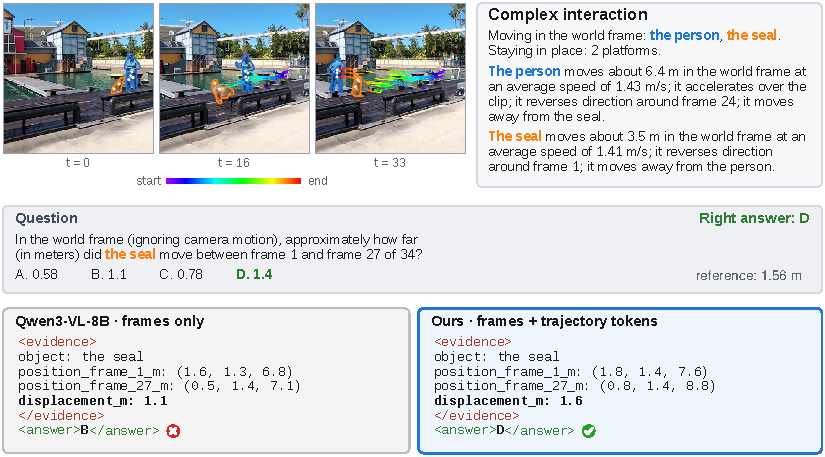
\includegraphics[width=\linewidth]{fig4_complex_interaction_labels.pdf}
\caption{\textbf{Complex interaction.} \emph{Top left:} three frames with estimated keypoint trajectories (colour encodes time). \emph{Top right:} the rule-generated motion caption. \emph{Bottom:} seal displacement between frames 1 and 27 (reconstruction-derived reference 1.56~m): frames only 1.1~m (wrong), frames and trajectory tokens 1.6~m (correct).}
\label{fig:qual-interaction}
\end{figure}

\begin{figure}[t]
\centering
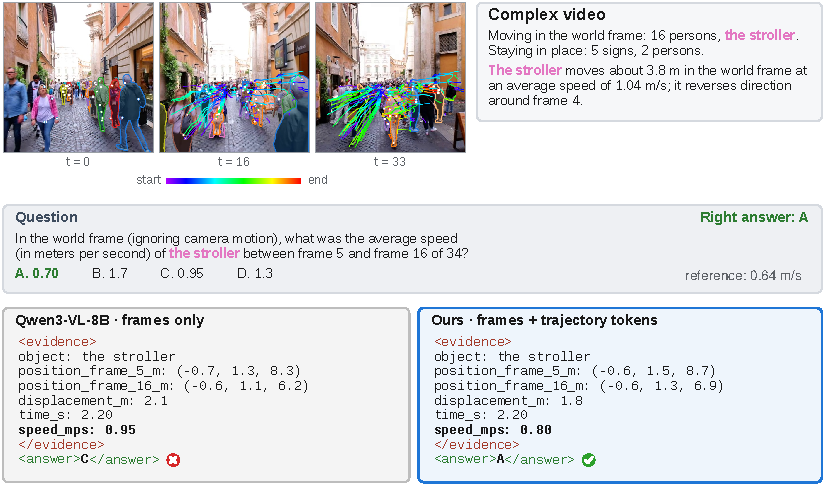
\includegraphics[width=\linewidth]{fig4_complex_video_labels.pdf}
\caption{\textbf{Complex video.} Same layout as Fig.~\ref{fig:qual-interaction}. The stroller's endpoint displacement rate between frames 5 and 16 (reference 0.64~m/s): frames only 0.95~m/s (wrong), frames and trajectory tokens 0.80~m/s (correct).}
\label{fig:qual-video}
\end{figure}

\begin{figure}[t]
\centering
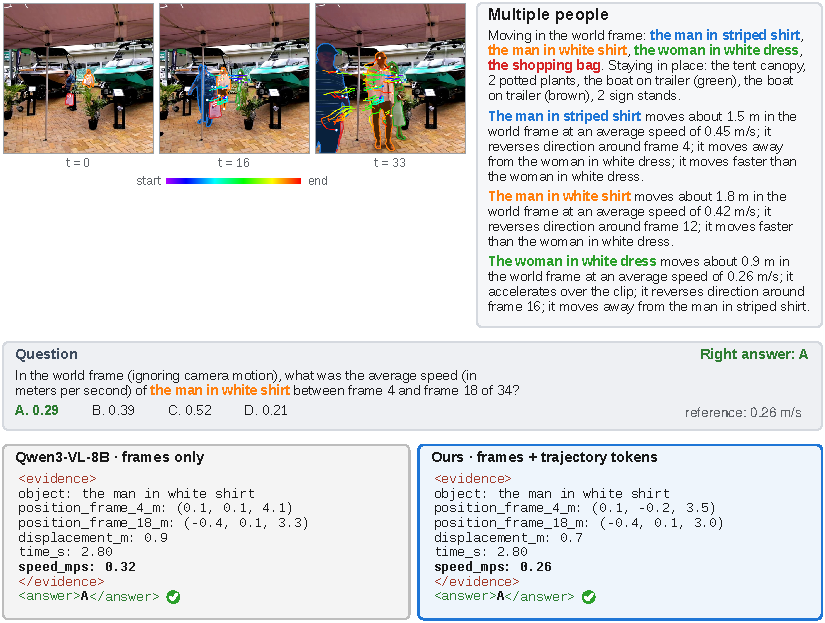
\includegraphics[width=\linewidth]{fig4_multiple_people_labels.pdf}
\caption{\textbf{Multiple people.} Same layout as Fig.~\ref{fig:qual-interaction}. The man's endpoint displacement rate between frames 4 and 18 (reference 0.26~m/s): both models answer correctly, frames only with 0.32~m/s and frames and trajectory tokens with 0.26~m/s.}
\label{fig:qual-people}
\end{figure}

\begin{figure}[t]
\centering
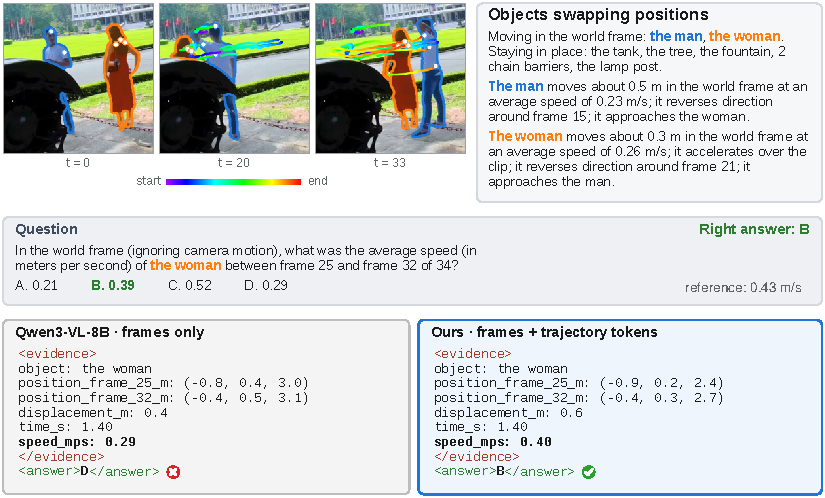
\includegraphics[width=\linewidth]{fig4_swapping_positions_labels.pdf}
\caption{\textbf{Objects swapping positions.} Same layout as Fig.~\ref{fig:qual-interaction}. The woman's endpoint displacement rate between frames 25 and 32 (reference 0.43~m/s): frames only 0.29~m/s (wrong), frames and trajectory tokens 0.40~m/s (correct).}
\label{fig:qual-swap}
\end{figure}

\clearpage
\subsection{Additional qualitative examples}
Five further selected clips are shown in Figures~\ref{fig:qual-approach}--\ref{fig:qual-horse}. Their embedded ``ground truth'' labels mean reconstruction-derived references, and any ``average speed'' question is scored as endpoint displacement divided by elapsed time. The cases illustrate answer and evidence differences; they are not a representative sample or component ablations.

\begin{figure}[H]
\centering
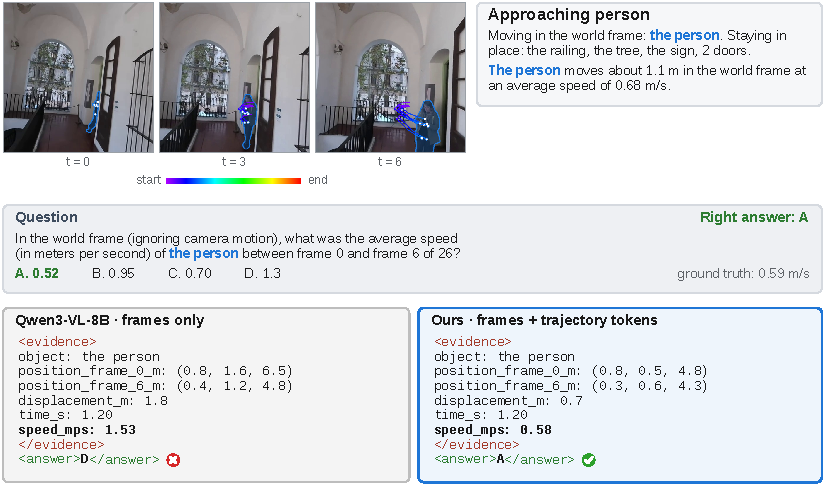
\includegraphics[width=\linewidth]{fig4b_approaching_person.pdf}
\caption{\textbf{Approaching person.} Endpoint displacement rate from frames 0 to 6: reconstruction-derived reference 0.59~m/s, frames-only evidence 1.53~m/s (wrong option), and trajectory-input evidence 0.58~m/s (correct option).}
\label{fig:qual-approach}
\end{figure}

\begin{figure}[H]
\centering
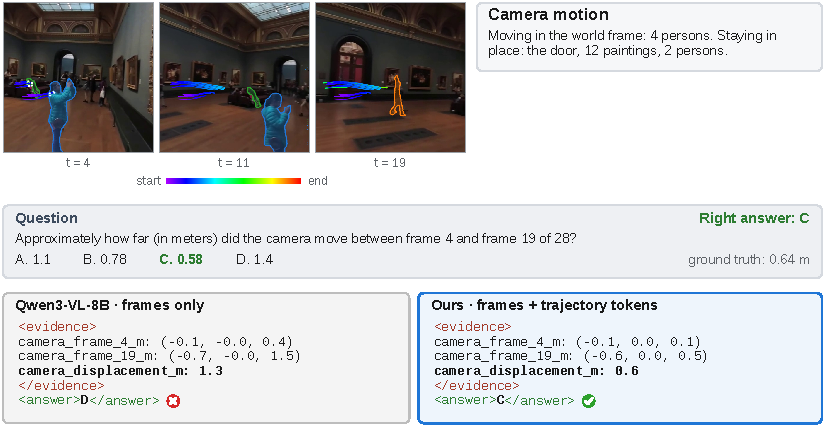
\includegraphics[width=\linewidth]{fig4b_camera_motion.pdf}
\caption{\textbf{Camera motion.} Camera displacement from frames 4 to 19: reconstruction-derived reference 0.64~m, frames-only evidence 1.3~m (wrong option), and trajectory-input evidence 0.6~m (correct option).}
\label{fig:qual-camera}
\end{figure}

\begin{figure}[H]
\centering
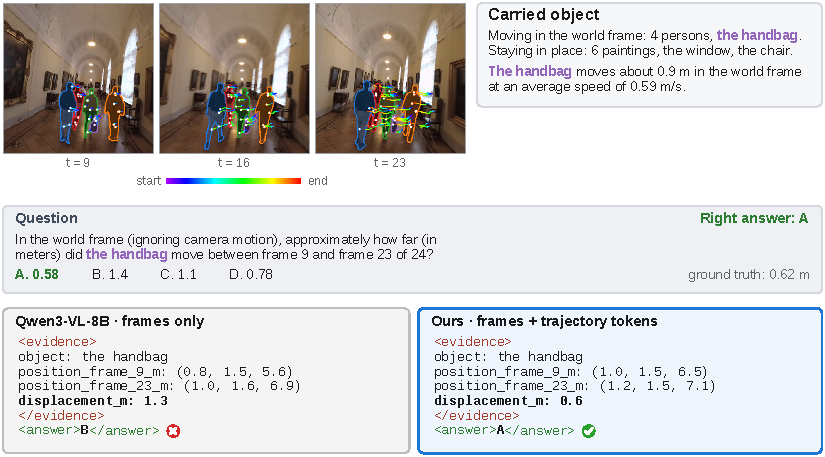
\includegraphics[width=\linewidth]{fig4b_carried_object.pdf}
\caption{\textbf{Carried object.} Handbag displacement from frames 9 to 23: reconstruction-derived reference 0.62~m, frames-only evidence 1.3~m (wrong option), and trajectory-input evidence 0.6~m (correct option).}
\label{fig:qual-carried}
\end{figure}

\begin{figure}[H]
\centering
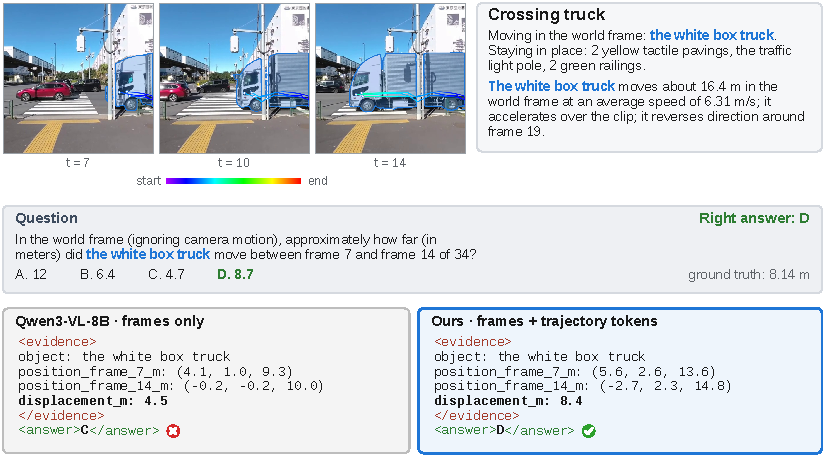
\includegraphics[width=\linewidth]{fig4b_crossing_truck.pdf}
\caption{\textbf{Crossing truck.} Truck displacement from frames 7 to 14: reconstruction-derived reference 8.14~m, frames-only evidence 4.5~m (wrong option), and trajectory-input evidence 8.4~m (correct option).}
\label{fig:qual-truck}
\end{figure}

\begin{figure}[H]
\centering
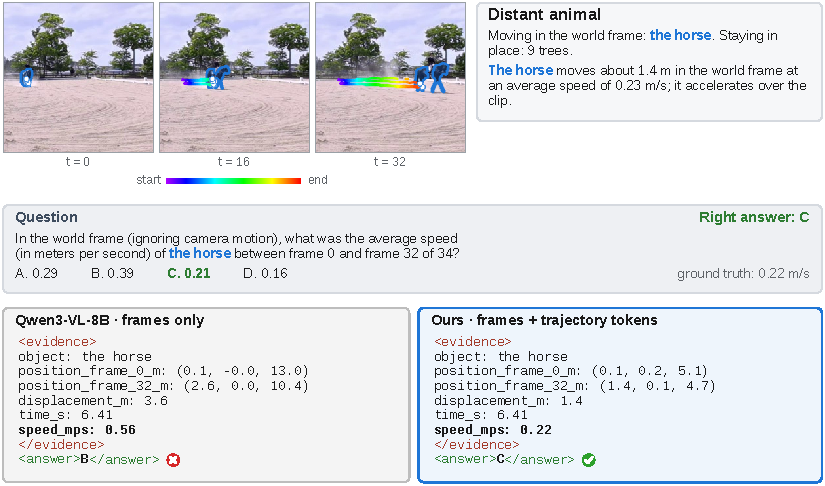
\includegraphics[width=\linewidth]{fig4b_distant_animal.pdf}
\caption{\textbf{Distant animal.} Horse endpoint displacement rate from frames 0 to 32: reconstruction-derived reference 0.22~m/s, frames-only evidence 0.56~m/s (wrong option), and trajectory-input evidence 0.22~m/s (correct option).}
\label{fig:qual-horse}
\end{figure}

\clearpage

\section{Limitations and Scope}
\label{app:limitations}
TrajQA-B is built from Stereo4D's reconstructed tracks. Its reference answers inherit errors in those tracks, masks, object assignments, and camera poses. Questions are deliberately defined to be answerable from the serialized records, so accuracy measures trajectory reading under this construction rather than recovery of 4D geometry from raw video or transfer to arbitrary motion tasks. Some original prompts use the phrase \emph{average speed} for endpoint displacement rate; this wording should be corrected when regenerating the benchmark. External baseline comparisons differ in supervision, visual processing, and sometimes evaluation subset. The separately trained frames-only arm is the closest visual comparison, but its full optimization schedule is unavailable and its eight sampled frames lack timestamps; queried endpoints may be absent. Stage-1 training excludes QA evaluation scenes, but its source-video and validation-set relation to QA evaluation has not been independently audited in the available records. Results use one training seed, and no experiment isolates the contribution of part labels, event splitting, adaptive spline fitting, or projector warm-up. Future evaluation should use independent motion ground truth, documented stage-1 source-video separation, matched frame and timestamp inputs, and component ablations.



\end{document}
